\documentclass{article}
\usepackage[english]{babel} % en
\usepackage{graphicx}
\usepackage{hyperref}
\usepackage[T1]{fontenc}
\usepackage[utf8]{inputenc}
\usepackage{setspace}
\usepackage[paper=a4paper,margin=1in]{geometry}
\usepackage{parskip}
\usepackage{fancyhdr}
\usepackage{cite}
\usepackage{units}
\usepackage[htt]{hyphenat}
\usepackage{enumitem}
\usepackage{wrapfig}
\usepackage{mathtools}
\usepackage{relsize}
\usepackage{listings}
\usepackage{xcolor}
\usepackage{amsfonts}

\title{Query Optimization}
\author{Ilaria Battiston \thanks{All notes are collected with the aid of material provided by T. Neumann. All images have been retrieved by slides present on the \href{https://db.in.tum.de/teaching/ws2021/queryopt/}{TUM Course Webpage}.}}
\date{Winter Semester 2020-2021}
\pagestyle{fancy}

\definecolor{azzurro}{cmyk}{1,0.33,0,0.13}
\definecolor{arancione}{cmyk}{0,0.41,1,0}
\definecolor{verde}{cmyk}{0.44,0,0.38,0.31}
\definecolor{viola}{rgb}{0.58,0,0.82}
\definecolor{bianco}{rgb}{0.95, 0.95, 0.92}
% C style
\lstdefinestyle{CStyle}{
    backgroundcolor=\color{bianco},   
    commentstyle=\color{verde},
    keywordstyle=\color{viola},
    numberstyle=\tiny\color{arancione},
    stringstyle=\color{azzurro},
    basicstyle=\footnotesize,
    breakatwhitespace=false,         
    breaklines=true,                 
    captionpos=b,                    
    keepspaces=true,                 
    numbers=left,                    
    numbersep=5pt,                  
    showspaces=false,                
    showstringspaces=false,
    showtabs=false,                  
    tabsize=2,
    language=C
}
\lstset{
  basicstyle=\ttfamily,
  columns=fullflexible,
  frame=single,
  breaklines=true,
  postbreak=\mbox{\textcolor{red}{\(\hookrightarrow\)}\space},
}

\graphicspath{{./images/}}

\sectionfont{\fontsize{18}{15}\selectfont}
\subsectionfont{\fontsize{15}{15}\selectfont}
\subsubsectionfont{\fontsize{12}{15}\selectfont}

\begin{document}

\maketitle

\lfoot{}
\cfoot{}
\rfoot{\thepage}

\newpage
\setcounter{tocdepth}{2}
\tableofcontents
\newpage
\section{Introduction}
A \textbf{cryptosystem} consists of a family of \textit{enciphering transformations} $f$, each corresponding to a choice of parameters $p$, from a set $P$ of all possible plaintext message units to a set $C$ of all possible ciphertext message units. The transformation requires:
\begin{itemize}
	\item An algorithm, which is the same for the whole family and supposedly publicly known;
	\item An enciphering key $K_E$, the value of parameters $p$;
	\item A deciphering key $K_D$.
\end{itemize}
The deciphering key is needed in order to compute $f^{-1}$, i.e.\ decipher the message. The transformation uses the same algorithm as encrypting, except with a different key. 

A \textbf{public key} or \textbf{asymmetric cryptosystem}, by definition, has the property that someone who knows only to encipher cannot use the encipher key to find the deciphering key without a prohibitively lengthy computation: the function $f : P \rightarrow C$ is easy to compute once $K_E$ is known, but it is very hard in practice to compute the inverse function $f^{-1} : C \rightarrow P$.

In mathematical terms, the inverse computation should be \textbf{infeasible}, namely so computationally intensive that it is impossible to evaluate it in any reasonable time period. 

This implies that $f$ is not invertible without some additional information, therefore $f$ is an \textit{one-way function}. Most public key algorithms are in fact based on number-theoretic functions, whose goal is usually not to have a compact mathematical description between input and output.

A public key cryptosystem, therefore, involves not only one key but a pair: one is public and can be publicly shared, and the other is private and its discover by a third part would compromise the security of the system.

The main point of this scheme is that it is not necessary that the key possessed by the person who encrypts the message is secret. Receivers can only decrypt using their secret key.

Information needed to send secret messages, therefore, can be made public without anyone being able to read the content. This makes communication possible within two parts which have never interacted before, an useful feature among modern systems with huge workloads. 

\subsection{Cyclic groups and generators}
\textbf{Cyclic groups} are a way to generalize public key algorithms within groups not necessarily constrained by a prime number. They have a key role in cryptography, since they allow many useful one-way functions which can be used to encrypt information: in fact, cryptographic functions which are hard to break should be defined within finite groups.

A \textbf{group} is a set of elements $G$ together with an operation $\circ$ which combines two elements of $G$. A group has the following properties:
\begin{enumerate}
	\item The group operation $\circ$ is \textit{closed}: for all $a, b \in G$, it holds that $a \circ b = c \in G$;
	\item The group operation is \textit{associative}: $a \circ (b \circ c) = (a \circ b) \circ c$ for all $a, b, c \in G$;
	\item There is an element $1 \in G$ called the \textit{neutral element} (identity) such that $a \circ 1 = 1 \circ a = a$ for all $a \in G$;
	\item For each $a \in G$ there exists an element $a^{-1}$ called the \textit{inverse}, such that $a \circ a^{-1} = a^{-1} \circ a = 1$;
	\item A group $G$ is \textit{abelian} (or \textit{commutative}) if, furthermore, $a \circ b = b \circ a$ for all $a, b \in G$.
\end{enumerate}
Cryptography majorly relies on \textit{multiplicative groups}, where the operation $\circ$ denotes multiplication.

Algorithms related to discrete logarithm problem, for example, concern the group $\mathbb{Z}^*_n$, consisting in the set of all integers $i = 0, 1, \dots, n - 1$ for which $\gcd(i, n) = 1$. $\mathbb{Z}^*_n$ forms an abelian group under multiplication modulo $n$, where the identity element is $e = 1$.

Since cryptography concerns finite structures, groups also have to respect the property to have a finite number of elements, defining the \textit{cardinality} or \textit{order} of the group $G$ by $|G|$. 

Every element of a group $G$ has also an order, which is the smallest positive integer $k$ such that:
$$a^k = a \circ a \circ \dots \circ a = 1$$
The $\circ$ operation is applied $k$ times, obtaining the identity element of $G$.

Example: the order of the element $a = 3$ in the group $\mathbb{Z}^*_{11}$ is 5, since $a^5 = 1 \mod 11$. 

The powers of $a$ run through the same finite sequence of remainders indefinitely, adopting a cyclic behavior. This allows to introduce cyclic groups.

A group $G$ which contains an element $\alpha$ with maximum order $|G|$ is said to be \textbf{cyclic}. Elements with maximum order are called primitive or \textbf{generators}, since every element $a$ of $G$ can be written as a power $\alpha^i = a$ of this element for some $i$, so that $\alpha$ generates the entire group.

For every prime $p$, $(\mathbb{Z}^*_p, \cdot)$ is an abelian finite cyclic group.

Having a finite cyclic group $G$, some interesting properties hold:
\begin{enumerate}
	\item For every $a \in G$, it holds that:
	\begin{enumerate}
		\item $a^{|G|} = 1$;
		\item The order of $a$ divides $|G|$;
	\end{enumerate}
	\item The number of primitive elements of $G$ is $\phi(G)$, where $\phi$ defines the Euler function (number of positive integers up to $G$ which are coprime to it);
	\item if $|G|$ is prime, then all elements $a \neq 1$ are primitive.
\end{enumerate}
Those concepts have relevancy in cryptography: prime fields are widely used for building discrete logarithm cryptosystems, using the fact that in a cyclic group \textit{only element orders which divide the group cardinality} exist. 

\subsubsection{Subgroups}
\textbf{Subgroups} are subsets of cyclic groups which are groups themselves, therefore respect all the previously stated properties. 

Let $(G, \circ)$ be a cyclic group. Then, every element $a \in G$ with $ord(a) = s$ is the primitive element of a cyclic subgroup with $s$ elements.

As previously stated, the generator can be non-unique. An important special case are subgroups of prime order: with cardinality $q$, all elements $e \neq 1$ have order $q$ as well.

If $H$ is a subgroup of $G$, then $|H|$ divides $|G|$. 

To obtain a construction method for subgroups from a given finite cyclic group, only the cardinality $n$ and a primitive element are needed: then, $\alpha^{n/k}$ is computed to obtain a generator $\alpha$ of the subgroups with $k$ elements.

This follows knowing that every integer $k$ which divides the cardinality $n$ there exists exactly one cyclic subgroup $H$ of $G$ of order $k$, consisting in the elements $a \in G$ satisfying $a^k = 1$. 



% !TeX root = ../notes.tex

\section{Textbook Query Optimization}
Textbook query optimization involves techniques to perform a rough first optimization, which however is quite simple. There is a series of steps to translate raw SQL into logical and physical plans, each of them transforming input in a more optimal form.

The output is going to be \textit{executable}, but still to be improved by non-trivial methods.

\subsection{Algebra and tuples}
Plain relational algebra is not sufficient itself: it needs to be revisited ensuring \textbf{correctness} (producing the same result) within a formal model. The most relevant problem to tackle is \textbf{deciding whether two algebraic expressions are the same}, but this in difficult in practice.

For instance, performing a selection before a join might be correct (and faster) in case the considered criterion is equality, but can give a different result than selecting after an outer join. 

To remedy this issue, it is possible to guarantee that two expressions are equivalent, not accepting false positing yet allowing false negatives. 

A formal definition of \textbf{tuple} is an unordered mapping from attribute names to values of a domain. A schema consists in a set of attributes with domain $A(t)$.

Tuple operations are:
\begin{itemize}
	\item \textbf{Concatenation}, attaching one tuple to another regardless of ordering (union);
	\item \textbf{Projection}, producing a notation $t.a$ in which it is possible to access single values or multiple $t_{|\{a, b\}}$, getting a subset of the schema.
\end{itemize}

A set of tuples with the same schema forms a \textbf{relation}. Sets naturally do not comply with real data, since they not allow duplicates, but are used for simplicity.

In most cases, sets and bags can be used interchangeably, but the optimizer considers different semantics: logical algebra operates on \textit{bags}, physical algebra on \textit{streams} and sets are only considered after an \textit{explicit duplicate elimination}.

\begin{figure}
	\begin{minipage}{0.45\textwidth}
		\hspace{-2mm}
		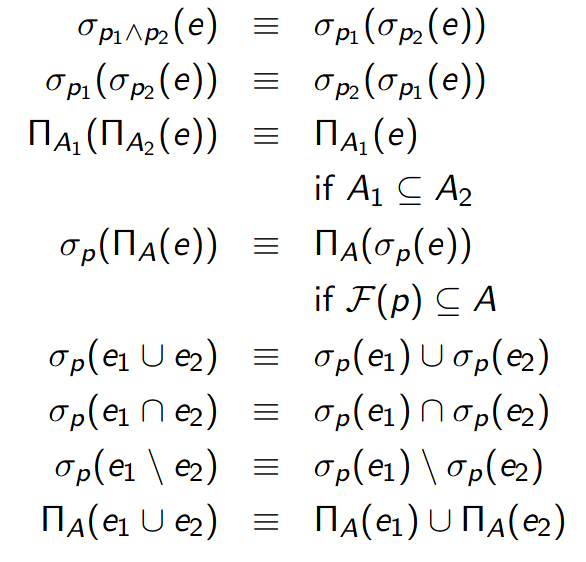
\includegraphics[width=0.83\textwidth]{equivalences_1.png}
	\end{minipage}
	\begin{minipage}{0.5\textwidth}
		\hspace{-10mm}
		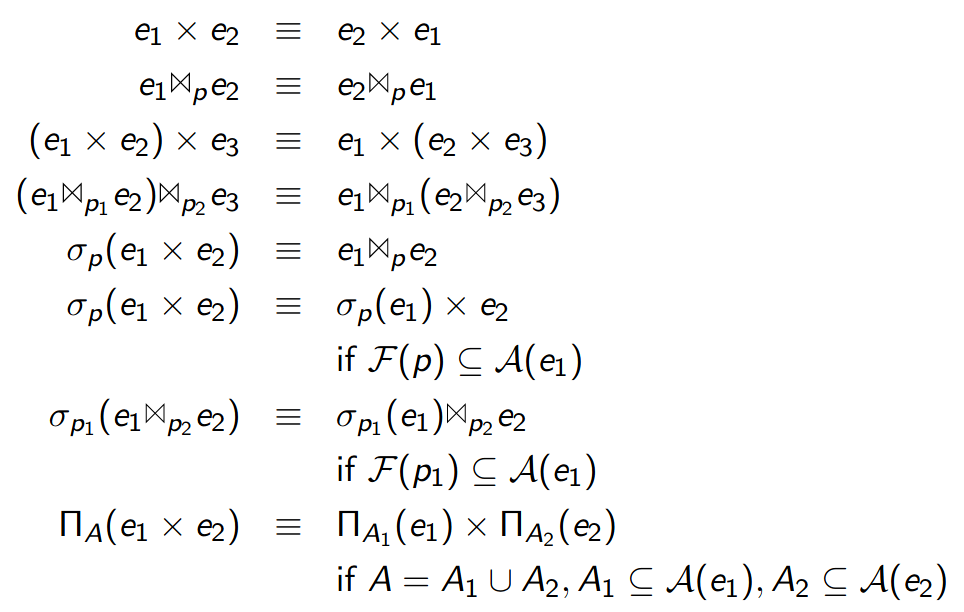
\includegraphics[width=1.2\textwidth]{equivalences_2.png}
	\end{minipage}
	\vspace{-15pt}
\end{figure}

Set operations are the classic ones of union, intersection and difference, yet are \textbf{subject to schema constraints}. On bags, operations are performed on frequencies. 

There are also \textit{free variables}, which first must be bounded to be evaluated: they are essentials for predicates and algebra expressions, such as dependent joins. 

It is important to note that projection removes duplicates within sets, while keeping them in bags.

There are equivalences for selection and projection useful to derive whether a different ordering produces the same output. For instance, applying selection twice is the same as applying it once with two criteria plus an AND. Commutative property also holds.

\subsection{Canonical Query Translation}
Canonical query translation transforms SQL into \textbf{algebra expressions}. The first approach involves some restrictions: it assumes no duplicates without aggregation and set operations.

The first step is translating the FROM clause:
$$F = \begin{cases}
R_1 & k = 1 \\
((\dots (R_1 \times R_2) \times \dots) \times R_k)) & \text{else}
\end{cases}$$
In short, all relations are joined through a cross product. The next step is translating the WHERE clause:
$$W = \begin{cases}
F & \text{there is no WHERE clause} \\
\sigma_p(F) & \text{otherwise}
\end{cases}$$
The SELECT clause is translated starting from the projection $a_1,\ \dots,\ a_n$ or $*$. The expression is constructed:
$$S = \begin{cases}
W & \text{if the projection is ALL} \\
\prod_{a_1,\ \dots,\ a_n}(W) & \text{otherwise}
\end{cases}$$
GROUP BY can also be translated, even though it is not part of the canonical translation. Let $g_1,\ \dots,\ g_n$ be the attributes in the clause and $agg$ the aggregations within SELECT:
$$G = \begin{cases}
W & \text{there is no GROUP BY clause} \\
\Gamma_{g_1,\ \dots,\ g_m:agg}(W) & \text{otherwise}
\end{cases}$$
HAVING is basically the same as WHERE, with the filter predicate on top of $G$.

\subsection{Logical Query Optimization}
Once obtained the relational algebra, equivalences span the \textit{potential search space} and new expressions are derived thanks to them. Of course equivalence can be applied both ways, hence it is relevant to decide which one works better, and conditions have to be checked as well. This, however, makes the search more expensive since there are plenty of alternatives.

To speed the process up, sometimes some equivalences are ignored, even the simplest ones (for instance when choosing the join algorithm).

Query plans can only be compared if there is a cost function, often needing details which are not available merely through relational algebra (what kind of join is being used): logical query optimization is still a \textbf{heuristic} and requires additional steps, since it is not enough to determine the runtime.

Most algorithms, therefore, use the following strategy:
\begin{itemize}
	\item Organization of equivalences into \textbf{groups};
	\item \textbf{Directing equivalences}, deciding the preferred side and rewriting rules to apply them sequentially to the initial expression, trying to reduce the size of intermediate results.
\end{itemize}
For example, a projection on the output of a join can be preferred to a join of a projection. It is important to keep in mind that tuples are being removed in the process, and this only applies in certain circumstances (regular expressions, high selectivity of join).

The rule of thumb is simply to eliminate the most tuples during the intermediate step, to then perform computationally expensive operation with the smallest amount of data.

To summarize, the phases are:
\begin{itemize}
	\item Breaking up conjunctive selection predicates, since simpler predicates can be moved around easier;
	\item Pushing selections down, reducing the number of tuples early;
	\item Introducing joins, which are cheaper than cross product (linear time);
	\item Determining join order, a usually NP-hard problem which is tackled with different approaches;
	\item Introducing and pushing down projections, removing redundant attributes.
\end{itemize}
Some SQL queries have limitations: selections sometimes cannot be pushed down, since there might be no join predicate between tables (cross product). Choosing a different join order allows further push down. 

\subsection{Physical Query Optimization}
Physical query optimization adds execution information to the plan, allowing actual cost calculation and optimizing over data structures, access path and operator implementation.

Data may be sorted or materialized, introducing results which can be reused and deciding where to store them.

First of all, the access path is selected: lookup can be done through \textbf{index} or \textbf{table scan}, depending on the selectivity (fraction of the data satisfying the clause): in general, above 10\% a table scan is recommended. 

Scanning a table might be efficient since tuples are stored \textit{adjacent} in memory; using index, instead, involves traversing a tree multiple times starting from the root. 

Sometimes it is useful to just store in cache the output of a view, but that also depends on the query plan: intermediate results should actually be reused.

\textbf{Operator selection} is replacing a logical operator with a physical one, according to semantic restrictions (most operators require equi-join).

A blockwise nested loop join is generally better than a natural join; sort merge join and hash join are better than both. In general, hash join is the best if not reusing sorts. This process must be performed for all operators: sort join requires ordered tuples, distributed databases need local data and there are multiple ways to model the properties (hashing).

Sort merge join might outperform the hash join if the amount of data is much larger than the available memory.

\textit{Materializing}, on the other side, is quite relevant for nested loop joins: the first pass is expensive, but the afterwards ones are way cheaper, making it essential for multiple consumers. 

\section{Join Ordering}
Join ordering focuses on conjunctive queries with simple predicates of the type $a_1 = a_2$ where the latter can be either an \textbf{attribute} or a \textbf{constant} (commonly used algorithms assume join between \textit{attributes}).

Relations may include selections or complex building blocks, however for simplicity filtering is ignored; having operators other than equality might cause differences within the query planner.

Ordering basically means choosing \textit{which relation to be joined first}, placing entities in a graph and adding an edge whenever a predicate from a node is joined to another. 

This kind of schema is defined as a \textbf{query graph}, in which edges consist in predicates and self loops represent equality with a constant. Usually cycles are pushed down, since algorithms only assume attributes. 

Based on the query graph it is possible to obtain an overview of the complexity of the problem: there are different shapes which are treated differently. 

\begin{figure}[h]
	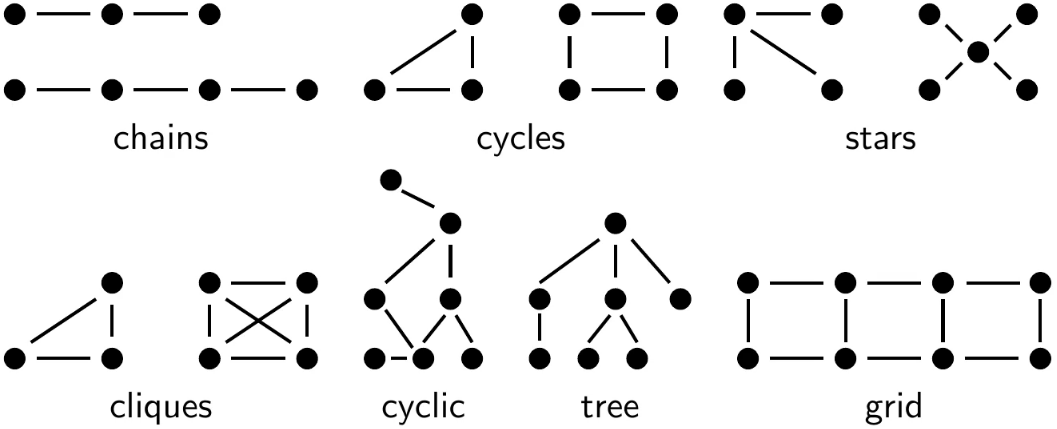
\includegraphics[scale=1.5]{query_graph.png}
	\centering
\end{figure}

\begin{enumerate}
	\item \textbf{Chains} are the simplest kind of query, fairly common in practice;
	\item \textbf{Cycles} (cyclic) are a chain with a closing edge, the easiest example of cycles;
	\item \textbf{Stars} are mostly used in data warehouse, in which the center table has large dimension and the ones outside are relatively small, quite different to solve;
	\item \textbf{Cliques} are instances in which every relation is joined with all the others, and are the hardest to optimize causing the worst runtime;
	\item \textbf{Trees} are acyclic queries even if the level of nesting can be high;
	\item \textbf{Grids} are also fairly hard and interesting for research.
\end{enumerate}

Joins are represented with \textbf{join trees}, binary trees with operators as inner nodes and relations as leaves. The most common type is unordered (not distinguish left from right) without cross product, however algorithms might produce other variants.

There furthermore are different kinds of trees:
\begin{itemize}
	\item \textbf{Left-deep} tree, in which joins only happen on the left side, easy to represent and implement through hash tables ($n!$ trees with cross products);
	\item \textbf{Right-deep} tree ($n!$);
	\item \textbf{Zig-zag} tree, a combination of the previous ($n!2^{n-2}$);
	\item \textbf{Bushy} tree, a full binary tree (non-linear, harder to find optimal solutions but can be the most efficient in some cases, $n!C(n-1) = \frac{(2n-2)!}{(n-1)!}$ where $C$ represents a Catalan number).
\end{itemize}
It is relevant to notice that the number of leaf combinations and unlabeled trees grows \textbf{exponentially}, and increases even more with a flexible structure. However, nodes can often be swapped from left to right.

Another important information about joins is their \textbf{selectivity}, the amount of tuples which will result from an equivalence between two attributes: 
$$f_{i, j} = \frac{\abs{R_i \bowtie_{p_{i, j}} R_j}}{\abs{R_i \times R_j}}$$
This depends on whether the attributes are a key, and gives an estimation of the result cardinality with the aid of assumptions and statistics.

Given a join tree, the \textbf{cardinality} (size of the cross product) can be computed recursively as the productory of the selectivity function multiplied by the size of both relations. This allows easy calculations only requiring base cardinalities and independence of predicates:
$$C_{out}(T) = \begin{cases}
0 & T\text{ is a leaf} \\
\abs{T} + C_{out}(T_1) + C_{out}(T_2) & T = T_1 \bowtie T_2
\end{cases}$$
This formula sums up the sizes of intermediate results, which are the ones causing more works. There are basic specific cost functions for joins, to be summed to the cost of single relations. 

Algorithms are mainly designed for left-deep trees, and some of the cost functions do not work in practice, for instance in the case of cross products. Therefore, those indicators are mainly theoretical and work under strict assumptions. However, join ordering is a main factor \textit{regardless of the chosen cost methods}.

Most of the time, algorithms for query optimization tend to avoid cross products, despite the enormous number of possibilities to build a join tree: the only exception regards small relations.

\subsubsection{Symmetry and ASI}
A cost function is called symmetric if $C_{impl}(e_1 \bowtie^{impl} e_2) = C_{impl}(e_2 \bowtie^{impl} e_1)$. Commutativity can be ignored.

ASI (Adjacent Sequence Interchange) are a set of properties characterizing simple cost functions, consisting in swapping two adjacent sequences with a larger one. They are relevant since some operations should be performed before others, to optimize costs. 

\textit{Let \textbf{f} be ASI with rank function \textbf{r}, and let $\vec s$ and $\vec t$ be strings. Consider a job module $\{\vec s, \vec t\}$ in a general precedence graph, where $\vec s \rightarrow \vec t$ and $r(\vec t) \leq r(\vec s)$. Then there is an optimal permutation with $\vec s$
immediately preceding $\vec t$.}

This property will be exploited in one of the most famous join ordering algorithms (IKKBZ), which heavily relies in swapping sequences.

\subsubsection{Chains}
Chains usually originate a left-deep tree: leaves can be ordered according to different degrees of freedom, as long as all the relations are joined. 

The number of possible left-deep trees can be defined recursively:
$$\begin{cases}
f(0) = 0 \\
f(1) = 1 \\
f(n) = 1 + \sum_{k=1}^{n-1} f(k-1) \cdot (n - k)
\end{cases}$$
Adding $R_n$ to all possible join trees can be done at any position following $R_{n-1}$. There are $n - k$ join trees for $R_n$, plus one assuming it can be placed before $R_{n-1}$ in the case of $k=1$. For $R_{n-1}$ to be at $k$, $R_{n-k} - \dots R_{n-2}$ must be below it.

Solving the recurrence gives the closed form $f(n) = 2^{n-1}$, still exponential yet much smaller than the case with cross products.

A generalization to zig-zag can be made expecting the same result.

Bushy trees, on the other hand, are not so easy to obtain: each subtree must contain a subchain to avoid cross products, hence single relations should not be added. It is possible to create a whole chain $R_1 - \dots R_n$, cut it and place it under another subtree, always considering commutativity.

This gives the formula:
$$ f(n) = \begin{cases}
1 & n < 2 \\
\sum_{k=1}^{n-1} 2f(k) \cdot f(n-k) & n \geq 2
\end{cases}$$
Having more than 2 relations implying performing a cut at some point $k$ and placing $k$ on the left side, $n - k$ on the right side. A factor of 2 indicates swapping the two sides. 

This gives the closed form $f(n) = 2^{n-1}C(n-1)$.

\subsubsection{Stars}
Star queries have the constraint that \textit{one relation must be in the center}; all the others can be ordered arbitrarily. This leads to the following formulas:
\begin{itemize}
	\item Left-deep: $2 \cdot (n - 1)!$, since there are $n - 1$ choices for a join partner and a factor of 2 for commutativity;
	\item Zig-zag: $2 \cdot (n - 1)! \cdot 2^{n-2}$, in which the last factor represent the possibility to swap left and right for each subtree;
	\item Bushy trees: not possible since they require the first relation to be available. 
\end{itemize}

\subsubsection{Cliques}
Cliques are a schema which do not care about cross products, since every relation is connected to the other, hence the number of possibilities is the same as the one obtained allowing cross products. 

Still, complexity is very high and runtime is bad, although the worst case usually does not happen. 

\subsection{Greedy heuristics}
Regardless of the methods and the inclusion of cross products, the search space is in general quite large when the number of relations is larger than 10, and polynomial time is hard to achieve. Some cost functions do not even have a proof of complexity.

Due to the size of the search space, \textit{greedy heuristics} are ways to easily construct a potential tree in a fast time: they are most suitable for \textbf{large queries}, but often do not give the best result.

This class of algorithms assumes no cross products within left-deep trees, and known cardinalities (or some other weight function).

\subsubsection{GreedyJoinOrdering-1}
This algorithm returns a set of ordered relations to be joined according to a cost function in a bushy tree structure, which in this case is the size of each node. 

The output is given starting from the \textbf{minimum-weight relation}, removes it and searches for the new minimum. 

This method is simple, but not that good in practice: it assumed fixed weight (not depending on the size, for instance) and does not support optimization within intermediate results. 

\subsubsection{GreedyJoinOrdering-2}
This variant also considers the \textbf{previous set of relations}, computing relative weights based on the existing tree. The only difference with the first version is the computation of minima considering also previous results.

It works picking the first relation based on cardinality, and all others according to minimum selectivity. In this case, however, the very first relation has a large relative weight and a major impact on the choices made afterwards. 

\subsubsection{GreedyJoinOrdering-3}
To tackle the problem introduced by the second version, a double loop is employed in which not only the set of relations is scanned, but also every relation is tested as a starting one. Then, all computed results are compared and the minimum among them is returned. 

This method is overall the best one and is implemented in some systems, but it is still not optimal.

\subsubsection{Greedy Operator Ordering}
This algorithm is a more complicated heuristic approach allowing to find \textbf{bushy trees}, while the others are limited to left-deep shapes, taking advantage of semantic information to produce a good join ordering.

Intermediate join trees must be combined in a bottom-up way to obtain larger trees: since some algorithms construct left-deep structures and others return bushy trees, those can be attached if the result is minimal: trees with the smallest weight are iteratively joined and then removed by the set of possibilities. 

The core idea is to \textit{always perform the most profitable joins first}, according to the size of intermediate results, taking into account earlier steps as well and aiming to lower the cost of intermediate results. After two nodes are selected from the query graph, GOO always updates it to reflect the new cardinalities and selectivities.

The algorithm constructs an optimal operator tree by \textbf{merging pairs of graph nodes}. First, each combination of weight (for instance, product of cardinalities and selectivity) is calculated; then the minimum is chosen and the two relations are aggregated into a new one, changing related edges. 

In case both relations are linked to the same (different) one in the query graph, the selectivity of the new edge consists in the product of previous ones. The process is iteratively repeated until only one node is left. 

This algorithm has two pitfalls: one is its computational complexity of $O(n^3)$, which however can be in the order of milliseconds with small input, and the other is its suboptimal output in some cases.

It is not possible to speed the execution up through auxiliary data structures such as the heap, since weights are modified at each iteration. Furthermore, it is not guaranteed that Greedy Operator Ordering finds the best bushy tree given a set of relations, even if it tends to have better results than the greedy ordering techniques.

\subsection{IKKBZ}
IKKBZ is a \textbf{polynomial time} algorithm for join ordering without cross products, producing \textbf{left-deep trees} under some assumptions: \textit{acyclic graphs, ASI cost functions and a fixed join technique}. It was built in two phases: IK, the first proposal, and IKKBZ, the improved version which is currently used.

The general idea is considering each relation as starting point, trying to obtain a benefit ordering based on a rank function, and constructing compounds if any set violates ordering rules.

The algorithm will ultimately compute a \textit{rank} for each predicate, based on its selectivity, obtaining an optimal evaluation order. After the first steps, however, the remaining arguments are independent on the size of the relations.

It starts considering a cost function as a product of the form:
$$C(T_i \bowtie R_j) = \abs{T_i} \cdot h_j(\abs{R_j})$$
Each relation $R$ can have its own $h$ (cost for each relation), which has a set of parametrized cost functions $C_H$ (cost for a join). Cardinalities are also taken into account, defining $n_i = \abs{R_i}$ and $h_i(n_i)$ as the cost per input tuple of a join. $T_i$ is the left side of the computation.

A \textbf{predecence graph} helps identifying which relations should be joined first; it is represented as an oriented query graph, and constructed with root in $R_k$ in the following way:
\begin{enumerate}
	\item The root is fixed, removed by the set of possibilities and added to the tree;
	\item As long as there are relations to be chosen, $R_i \in V \setminus V_k^P$ is selected such that $\exists\ R_j \in V_k^P : (R_j, R_i) \in E$;
	\item $R_i$ is added to $V_k^P$ and an edge $R_j \rightarrow R_i$ is created.
\end{enumerate}

Remainder: the algorithm constructs left-deep trees.

Next steps of the algorithms consist in checking whether the nodes respect properties. A sequence of nodes conforms to a precedence graph if two conditions are satisfied:
\begin{itemize}
	\item For each position $i$ aside from the first, there exists one $j$ coming before;
	\item There does not exist a position $i$ and a $j$ coming after with an edge from $j$ to $i$ (acyclic).
\end{itemize}

If there exists a path between two sets $R_i$ and $R'_i$, all relations from the first must be joined first; there is no join condition between any pair of relations aside from the one joining the two sets, hence the selectivity is 1.

Selectivity of the join:
$$s_i = \begin{cases}
1 & \abs{R_i'} = 0 \\
\prod_{R_j \in R'_i} f_{i, j} & \abs{R'_i} > 0
\end{cases}$$
In case of cycles, the selectivity cannot be uniquely determined: there could be two relations with different values. Therefore, first the precedence graph is fixed, and then selectivities are calculated.

If the query graph is a chain (total order), then the following properties hold:
$$n_{1, 2, \dots, k} = \prod_{i=1}^{k}s_in_i$$
$$C_H(G) = \sum_{i=2}^{n}\big[n_{1, 2, \dots, i-1}h_i(n_i)\big] = \sum_{i=2}^{n}\Big[\Big(\prod_{j=1}^{i}s_jn_j\Big)h_i(n_i)\Big]$$
The cardinality of the joins is equal to the productory of each selectivity for each cardinality among all relations.

If the \textbf{weight function} is indeed the \textbf{selectivity}, then $C_H \equiv C_{out}$. The factor $s_in_i$ determines how much the input relation changes its cardinality before further joins, and can be increasing or decreasing.

The algorithm employs a recursive definition of the cost function:
$$\begin{cases}
C_H(\epsilon) = 0 \\
C_H(R_i) = 0 & \text{the relation is the root} \\
C_H(R_i) = h_i(n_i) & \text{else} \\
C_H(S_1S_2) = C_H(S_1) + T(S_1) \cdot C_H(S_2)
\end{cases}$$
$$T(\epsilon) = 1 \qquad \land \qquad T(S) = \prod_{R_i \in S}s_in_i$$
Last $C_H$ definition corresponds to the cardinality performing all the relation in the sequence (the term $T$) and multiplying for the cost of last element.

This allows to use \textit{ASI properties}: in fact, these hold if and only if there exists a function $T$ and a \textbf{rank function} defined as:
$$rank(S) = \frac{T(S) - 1}{C(S)}$$
The following must hold:
$$C(AUVB) \leq C(AVUB) \leftrightarrow rank(U) \leq rank(V)$$
In other words, ASI properties hold if and only if the relations can be ordered by rank. The previously defined cost function can be proven to respect these constraints.

It is possible that the rank contradicts the precedence graph: the following definition is introduced to counter this occurrence.

Let $M = \{A_1, \dots, A_n\}$ be a set of sequences of nodes. Then $M$ is called a module if, for all sequences $B$ that do not overlap with the sequences in $M$, one of the following conditions holds:
\begin{itemize}
	\item $B \rightarrow A_i, \forall\ A_i \in M$;
	\item $A_i \rightarrow B, \forall\ A_i \in M$;
	\item $B \nrightarrow A_i \land A_i \nrightarrow B, \forall\ A_i \in M$.
\end{itemize}

If $A \rightarrow B$ and $rank(B) \leq rank(A)$, then it is possible to find an optimal sequence among those in which $B$ directly follows $A$.

If the precedence graph contains $A \rightarrow B$ but $rank(A) \geq rank(B)$, there is a so called \textbf{contradictory sequence}, and the two are combined, updating other edges by multiplying the cardinalities and selectivities. 

The continued process of building a compound relation until no more contradictory sequences exist is called \textbf{normalization}; the opposite is \textbf{denormalization}.

IKKBZ works performing the following steps for each relation, considering it as a root node:
\begin{enumerate}
	\item Calculates the precedence graph;
	\item Executes the subprocedure of finding the subtree all of whose children are chains, and normalizing it, then merging the chains;
	\item The relation returned by the previous step is added to the set.
\end{enumerate}
The algorithm stops when all trees are single chains, then returns the minimum of the sets according to the cost function.

The subprocedure constructs a left-deep tree (chain) from the precedence graph, performing a normalization operation and merging based on the rank in ascending order. Normalization happens when there is a contradictory sequence, i. e. one chain has bigger rank than the following.

This works by taking $r$ and $c$ such that $rank(r) > rank(c)$ and swapping them with a compound relation representing both. This allows to merge relations that would have been reordered if only considering the rank, obtaining the actual ascending order.

In case the graph contains cycles, it is possible to preprocess it with algorithms such as Minimum Spanning Tree to find a suitable representation to run IKKBZ.

\subsubsection{IK}
IK was originally proposed as a heuristic algorithm to minimize the number of page fetches necessary to evaluate a nested loop query in a database, providing a suboptimal solution to a NP-complete problem. 

The paper states the impossibility to solve optimization of the expected number of accesses, yet it determines the solution in the special case in which a query is a tree. 

Sorting each relation once gives an useful advantage since it decreases the number of pages in which tuples are looked for: if $T_i$ satisfies an attribute, $T_{i+1}$ will likely do it too, and it will be stored right below. This saving usually compensates the cost to sort.

The $H_i$ in this case is the total \textbf{number of page fetches}, and all other formulas are similar, taking advantage of pointers and approximation in practice to estimate actual costs.

Once found a somewhat accurate cost function, the problem of finding an optimal nested structure is divided into:
\begin{enumerate}
	\item Finding a nesting order;
	\item Finding a compatible directed spanning tree.
\end{enumerate}

A brute force approach would take up to $n!$ permutations into account, which is not feasible: a criterion must be imposed, generally the lexicographical order of the costs of each relation, in which $H$ should be the most dominant and uniquely determined.

For each relation in the query graph, the one minimizing $H$ is chosen and removed from the set, along with its incident edges, and the final order of choices is returned. This generates a \textbf{spanning tree}, hence removes all the cycles, in $O(n^3)$. 

Tree queries are a special case in which \textbf{direction of edges} is used as ordering constraint: if there is a path between two nodes, then the first must be ordered before the second. The minimization problem then becomes equivalent to minimizing the sum of all cost functions, taken in the best order.

Thanks to ASI properties, an optimal sequence can be obtained in $O(n\log n)$ when the constraints have the form of a directed tree. The algorithm repeatedly finds a \textbf{wedge}, i. e. two chains joined together at the end, and merges it to get a new chain, until it ends up with only one. At each iteration, a node keeps a well-defined rank regardless of its representation.

After the algorithm terminates, each node is again expanded by replacing it by the corresponding sequence of relations, ordered accordingly by their rank. 

Each node is considered as starting node, and the best solution over all is chosen, with a total computational runtime of $O(n^2\log n)$.

\subsubsection{KBZ}
KBZ is a variant of IK shown to be heuristically effective for cyclic queries as well, and works comparing different alternatives for each element of the search space. 

It improves IK since it supports different join methods, preprocessing and pushing selects, and it is also better in runtime: its worst case is $O(n^2)$, removing the logarithmic weight caused by the sorting.

This approach assumes a \textit{memory resident database}, i. e. there is no paging to disk during the execution. Once again, having the query graph as a tree defines a \textbf{partial ordering}: the root node must be joined first. 

Selectivity of each node here is explicitly defined as the selectivity of the join between it and its \textbf{parent}, since there is only one, and for the root it is unity: the consequence of this is, given the total ordering, a non-root relation joins with its parent first. Therefore, the best join method can be determined independently from the tree shape.

For a given tree derived by a query, therefore, two properties must hold for consistency:
\begin{itemize}
	\item The sequence is complied with the imposed partial order from the root;
	\item A join operation (not a cross product) must be performed at each non-leaf node.
\end{itemize}

Cost and computation of cardinality and selectivity remain the same as IK, yet the restrictions above and \textit{not having more than one temporary relation used in any join operation} limit the search space. 

However, the approach is slightly different: KBZ presents a method to find the optimal tree which is more efficient than computing the cost for each choice of the root. 

First of all, the original join tree is transformed so that the total order is respected, imposing that the root has only two children. The core idea is that computations corresponding to two choices for the root have a lot in common, especially if the roots are adjacent. 

Then, there is a phase of computing the rank of each relation, and merging in case of contradictory sequences. Cycles can be eliminated by considering the Minimum Spanning Tree.

\subsection{Maximum Value Precedence}
Maximum Value precedence is useful in those cases where IKKBZ fails, such as \textbf{cyclic queries}. It runs in polynomial time ($O(n^2)$) as well, employing a graph theoretic approach to calculate in how many ways joins can be scheduled.

This approach also provides a formal representation for operations of query and optimization parameters in an uniform manner, giving a cost once an execution plan is obtained in the form of a spanning tree.

The algorithm requires a weighted directed \textbf{join graph}, similar to the ones discussed before, which will be modified later, hence the definition must be extended: edges are assigned an \textbf{order}, and \textbf{predicates} (nodes) are used to identify sets.

In this representation, each node corresponds to a join, and a directed edge indicates the order of execution. If there exists an edge between the predicates $p_1$ and $p_2$, and they belong to the same relation, two directed edges are added in the graph.  

If $p_1$ is connected to $p_2$ and $p_2$ is connected to $p_3$, there will be a so called \textit{virtual edge} connecting $p_1$ and $p_3$: eventually, all nodes will be connected with either physical or virtual edges, forming a clique.

\begin{wrapfigure}{R}{0.45\textwidth}
	\vspace{-20pt}
	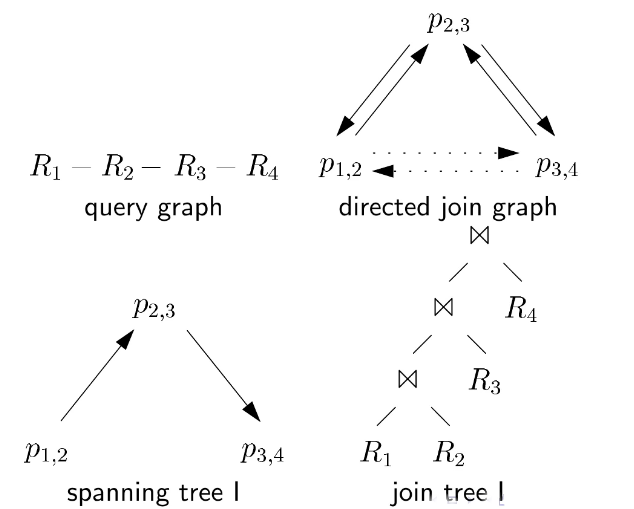
\includegraphics[width=0.48\textwidth]{MVP.png}
	\vspace{-30pt}
\end{wrapfigure}

For instance, \textbf{every spanning tree in the directed join graph leads to a join tree}: first of all edges are added in both direction, and then one of them gets removed, giving a directed acyclic graph which can easily give a join order (without distinguishing left and right).

MVP has the advantage of also producing bushy trees, however it does not guarantee optimality of the spanning tree; furthermore, the output might not correspond to an effective join tree, especially in uniprocessor environments.

Despite the incorrect representation, it is simple to fix this kind of errors, but there is no specific way to produce the best join tree.

To remedy the uncertainty, some additional rules are introduced to identify an \textbf{effective} spanning tree, which also help reducing the search space.

\textit{For a given query $R_1 \bowtie R_2 \bowtie \dots \bowtie R_n$, an effective spanning tree of this query is a directed binary spanning tree of its corresponding weighted directed join graph such that query result is obtained without requiring to execute any extra joins in addition to the joins of the spanning tree.}

The following conditions must be satisfied:
\begin{enumerate}
	\item $T$ must be binary (no nodes can have more than two children);
	\item For all inner connected nodes $(u, v)$, $R(T(u)) \cap R(v) \neq \emptyset$ (they must have predicates in common);
	\item For all $(u_1, v)$, $(u_2, v)$ one of the following holds:
	\begin{enumerate}
		\item $((R(T(u_1)) \cap R(v))) \cap ((R(T(u_2)) \cap R(v))) = \emptyset$ (they have a different relation in common);
		\item $(R(T(u_1)) = R(v)) \land (R(T(u_2)) = R(v))$ (the relations in common are the same between pairs).
	\end{enumerate}
\end{enumerate}
An effective spanning tree corresponds to a \textit{valid join tree}, despite the definition not being intuitive. Given this, the rest of the assumptions is simple: if every predicate involves two relations and an equi-join condition, then $R(u) \cap R(v)$ contains only a single relation.

Let $v$ be that relation, then $R_i \bowtie_v R_j$ is abbreviated by $\bowtie_v$.

The next step is adding weight to the edges, obtaining a weighted directed join graph. Each weight is calculated with the formula:
$$w_{u, v} = \frac{\abs{\bowtie_u}}{R(u) \cap R(v)}$$
This means that each edge has a weight depending on the relation they have in common and the first join cardinality. The intuition implies that if a join is \textit{executed before another}, the given relation becomes available and the edge weight can explain how the cardinality changes, i. e. how many tuples are generated.

This value can be bigger or smaller than 1, and can make the total cost bigger or smaller (the input size changes by a factor of $w_{u, v}$). For virtual edges, the weight is 1 by default. 

It is relevant to notice that the weight function used by MVP is the same one as $s_i$ in IKKBZ. However, it can also be chosen arbitrarily.

Of course, a weight smaller than 1 reduces the cost of following join operations. Furthermore, weights change over time depending on a partial spanning tree: 
$$w(p_{i, j}, S) = \frac{|\bowtie_{p_{i, j}}^S|}{\abs{R_i \bowtie_{p_{i, j}} R_j}}$$
$\bowtie_{p_{i, j}}^S$ is the result of the join after all joins preceding $p_{i, j}$ in $S$ have been executed. If the spanning tree is empty, the cost is merely equal to the cost of a simple join. 

\subsubsection{The algorithm}
The algorithm works in two phases:
\begin{enumerate}
	\item Taking the edges with weight smaller than 1, trying to reduce the work for latter operators as soon as possible;
	\item Adding the remaining edges, potentially causing an increase of the load, yet as late as possible.
\end{enumerate}
As a weighted directed join graph contains all execution plans of a query and each spanning tree corresponds to an execution plan, the task is to find the minimum cost. However, the minimum spanning tree algorithm cannot be directly applied, since the weights are not constant (they change after each modification). 

The rational is therefore reducing the expensive operations as early as possible. In order to meet this goal, two priority queues are introduced along with two phases, one with largest weights (phase 1) and one with smallest (phase 2). 

The working graph is initially just a set of predicates with no edges, and then the two phases are ran, sorting costs of vertices in descending order.

The first phase modifies the state of a working tree, taking the head of the first priority queue (the \textbf{most expensive}) and finding the joins which could make it cheaper, adding nodes with smaller weight while still keeping the graph acyclic. 

The working graph is updated, removing the edge and adding respective virtual ones until no edges can reduce costs, or there are no further nodes with weight less than 1.

In this case, the cheapest node is swapped from the first queue to the second; else, the edge to be added to the working tree will be the one which maximizes the difference within costs (minimizes the new cost). Weights are then recomputed. 

Phase 2 is called when the second queue is non-empty, again considering edges which respect the acyclic property. The procedure tries to minimize the additional cost caused by adding joins, finding edges causing minimum increase of the total result. 

The motivation behind phase 2 is that if an edge causes a large cost increase to its connecting join node, then the effect of this will propagate to all the rest join nodes; hence, these need to be considered as late as possible.

To effectively modify the working tree, an update function changes the state by performing unions of sets with edges and removal from the graph yet to consider. If there are two incoming physical edges, they are replaced with virtual ones. 

This also ensures the binary property, removing all cases in which a node could have two parents and handling eventual duplicates. However, there is still no guarantee of optimality. 

\subsection{Dynamic Programming}
Dynamic programming approaches can be useful to obtain more insights on possible orders with cost function. Since this kind of algorithm is a macro class, they can be defined on \textbf{any input} and give \textbf{any output} (bushy, left-deep).

These work thanks to an optimality principle: if an option is cheaper than another, \textit{the latter can be discarded} and the best solution is found only considering the set of further possibilities generated by the first.

Formally, let $T$ be an optimal join tree for relations $R_1, \dots, R_n$. Then, \textit{every subtree $S$ of $T$ is an optimal join tree for the relations contained in it}.

Despite some hypothetical concerns of suboptimality and the presence of physical properties which may alter the result, in practice this property holds.

\begin{wrapfigure}{L}{0.49\textwidth}
	\vspace{-10pt}
	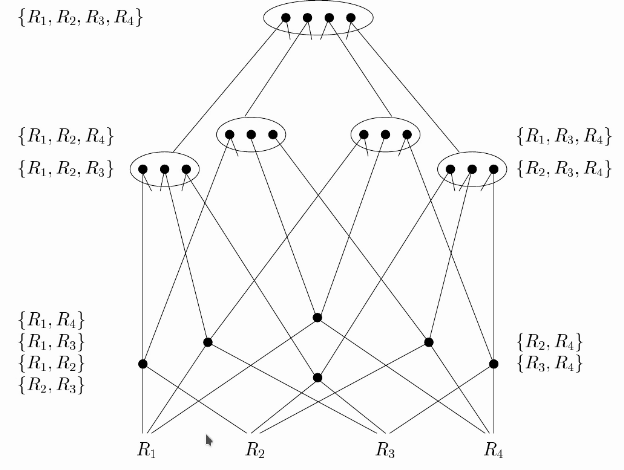
\includegraphics[width=0.5\textwidth]{search_space.png}
	\vspace{-40pt}
\end{wrapfigure}

The strategy works starting with a single relation and generating larger trees with a \textbf{bottom-up strategy}, reusing previous intermediate results.

A possible dynamic programming algorithm calculates the cost functions when joining either on the left or right side (bushy usually works better) for each applicable join implementation. 

The outcome will be a list of pairs with their cost, of which the minimum is chosen and propagated through following iterations.

The search space gets therefore reduced whenever an option is discarded, hence the number of combinations is never exponential.

\subsubsection{DPsize}
In the case of linear trees, there is a basic strategy which works finding the optimal $T$ by joining all optimal $T'$ with $T \setminus T'$, with $|T| = |T'| + 1$.

The most common algorithm is DPsizeLinear: it constructs the optimal \textbf{left-deep} tree from an empty table mapping the set of relations ($2^R$) to the join tree. 

For each relation, the optimal tree is built, starting from \textbf{size} 1 and increasing the subsets by adding those of smaller size having the optimal solution of the subproblem.

DPsize is an alternative approach which allows bushy trees as well: the only difference is that instead of adding one relation at the time, subsets can be joined.

If $S$ is a subset of $\{R_1, \dots, R_n\}$, before a join tree for it can be generated, the join trees for all relevant (valid) subsets of $S$ \textit{must already be available}.

For instance, if the query graph is a chain, before computing the optimal order there must be calculations for each connected pair, and of course for single relations.

DPsize can be made more efficient in case $s_1 = s_2 = \frac{n}{2}$: representing plans as a linked list, it is possible to iterate through it to retrieve all plans joining $s_1$ relations, and considering the succeeding ones for $s_2$, decreasing the complexity to $s_1 \cdot \frac{s_2}{2}$.

\subsubsection{DPsub}
DPsub is a dynamic programming alternative to DPsize, using \textbf{integer order}, a numeration used to order relations instead of the size (subset-driven).

This representation can be seen as a binary number in which a digit is 1 if the set contains the relation corresponding to its position, and 0 otherwise. For instance, having three relations, $011$ is $\{R_1, R_2\}$.

Integer order is used to fill the dynamic programming table, calculating all combinations for each $2 \leq i \leq 2^n-1$ and finding all subsets such that their \textbf{binary representation} is 1.

To get a labeling, an intuitive way is to perform a breadth-first search on the tree picking any arbitrary root (any labeling is however accepted).

The real implementation does not perform any mathematical operation, since each $i$ already represents a set. 

Then, for each relation in the subset, the cost is added to smaller subproblems, similarly to the previous approach. The last bit of the set gets removed after every iteration.

This algorithm has even better performance when creating bushy trees, and its advantage is the speed of binary calculations (bitwise and). 

Bushy trees can indeed be generated by combining two optimal trees (children of newly-found node). The dynamic programming principle holds.

A basic strategy is in fact just optimizing over subproblems and aggregating them: the approach is similar to linear trees, with the variant that the combined size of each pair of intermediate result must be equal to $\abs{S}$. Every relation must also appear once, hence $S_1 \cap S_2 = \emptyset$.

Connectedness must also be tested, since the relations might not induce a connected subgraph. This is performed by checking whether there is a join predicate between relations.

In practice, the number of subsets is exponential, and most of the time sizes are not compatible: a possible implementation uses a linked list of all combinations, and edits it according to the next operation.

\begin{wrapfigure}{R}{0.52\textwidth}
	\vspace{-27pt}
	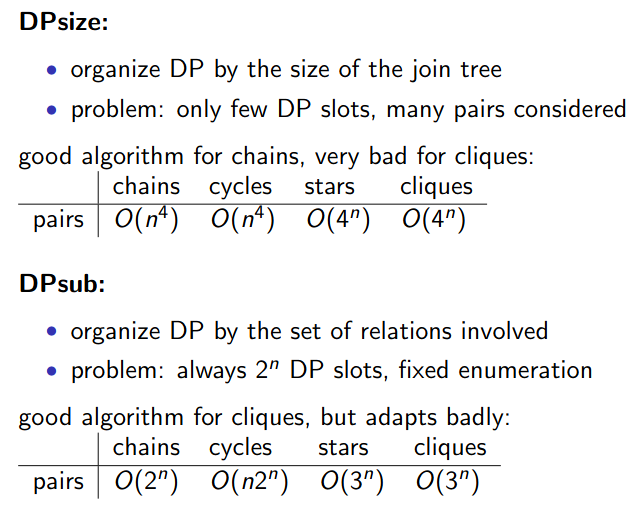
\includegraphics[width=0.52\textwidth]{dpsize_dpsub.png}
	\vspace{-100pt}
\end{wrapfigure}

Integer order is particularly efficient since the complement of a set ($S_2 = S \setminus S_1$) is found in constant time when the representation is binary.

All subsets can be enumerated as follows:
\begin{lstlisting}[language=C++]	S_1 = S & (-S)  // gives a number having only 1 as last bit
do {
	S2 = S - S1
	S1 = S & (S1 - S)  // same meaning as plus
} while (S1 != S)
\end{lstlisting}

Computational time is quite low, which is useful for a large amount of relations. However, it always depends on the number of combinations: DPsub is slower than DPsize in the polynomial case, and vice versa.

\subsection{Memoization}
Memoization is a top-down formulation of dynamic programming, \textbf{recursively} generating join tree in a way which allows to avoid duplicates and prune useless solutions.

Code is easier to understand and sometimes more efficient, but usually \textit{slower} due to recursiveness. However, it allows to generate bushy trees.

The memoization algorithm fills the table and then performs an auxiliary procedure for each subset: it checks whether the problem has \textit{already been computed}, otherwise it splits the subset in two and recursively calculates the two values. At the end of all function calls, the best value is picked between the two and cost is returned. 

The most performance-critical operation is the \textbf{lookup} in the hash table of known combinations, which can be expensive making the whole procedure slow.

The advantage is the knowledge of a \textbf{cost boundary} immediately after the first loop, meaning that in further iterations it is possible to propagate values so that more expensive plans can be discarded.

However, eliminating solutions might prune other optimal combinations or force suboptimal sets: the table must be extended, also remembering failures, so that it is not necessary to run the procedure another time.

The cost boundary can grow \textbf{exponentially}: a rule of thumb would be doubling it when searching for solutions and so on, ensuring a limited number of tries. 

\subsection{Connected subgraphs and DPccp}
For large queries, it is not quite efficient to construct subproblems which will be discarded later since they do not correspond to a valid tree. On the other side, it is possible to argue that pruning typically removes invalid subsets.

Having the query graph also helps to reduce asymptotic search space (polynomial) for chains, while it does not work well for cliques (exponential). Dynamic programming is instead better for cliques, but scales badly.

However, chains or quasi-chains are the most common kind of graph in real-world applications of joins, so the first approach is more useful in practice.

Connected subgraphs are another alternative to dynamic programming taking into account the \textbf{structure} of the query graph and the \textbf{connectivity} of nodes. 

This method is useful since, as previously stated, each variant of the two DP algorithms is superior to the other for one kind of query graph, but fails for the other, and neither is efficient for stars. Furthermore, it is very difficult to improve them while still excluding cross products.

Before introducing the algorithm, a few definitions should be stated:
\begin{enumerate}
	\item A connected subset is a connected subgraph induced by a subset of relations;
	\item \texttt{csg} is the number of non-empty connected subsets;
	\item A \texttt{csg-cmp-pair} (connected subgraph-complement) is a pair $(S_1, S_2)$ such that:
	\begin{itemize}
		\item $S_1$, $S_2$ are non-empty and connected;
		\item $S_1 \cap S_2 = \emptyset$;
		\item There exists $v_1 \in S_1$, $v_2 \in S_2$ such that there is an edge between $v_1$ and $v_2$;
		\item \texttt{ccp} is the number of csg-cmp-pairs;
	\end{itemize} 
\end{enumerate}
Of course, subsets should be also be connected with each other (a join predicate must exists) since cross products are to be avoided.

The approach aims to enumerate the number of connected subsets and csg-cmp-pairs, avoiding duplicates. There are some formulas which can be used with $n$ relations:
\begin{itemize}
	\item Chain queries:
	\begin{itemize}
		\item \texttt{csg}($n$) = $\frac{n(n+1)}{2}$;
		\item \texttt{ccp}($n$) = $\frac{(n+1)^3 - (n+1)^2 + 2(n+1)}{3}$;
	\end{itemize}
	\item Cycle queries:
	\begin{itemize}
		\item \texttt{csg}($n$) = $n^2 - n + 1$;
		\item \texttt{ccp}($n$) = $n^3 - 2n^2 + n$;
	\end{itemize}
	\item Star queries:
	\begin{itemize}
		\item \texttt{csg}($n$) = $2^{n-1} + n - 1$;
		\item \texttt{ccp}($n$) = $(n-1)2^{n-2}$;
	\end{itemize}
	\item Clique queries:
	\begin{itemize}
		\item \texttt{csg}($n$) = $2^n - 1$;
		\item \texttt{ccp}($n$) = $3^n - 2^{n+1} + 1$.
	\end{itemize}
\end{itemize}
Except for clique queries, the number of csg-cmp-pairs is orders of magnitude less than the search space for other DP variants.

The main idea is therefore only considering pairs of connected subproblems, more precisely the csg-cmp-pairs, which also corresponds to the \textbf{lower bound} of any dynamic programming algorithm. 

\begin{figure}[h]
	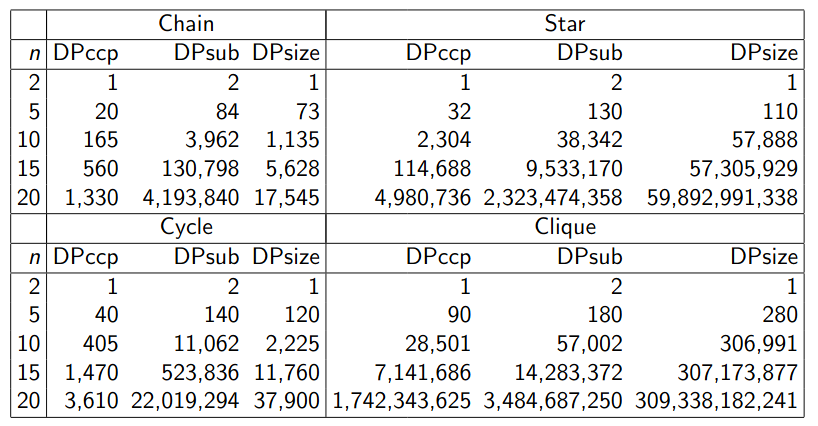
\includegraphics[scale=0.45]{dp.png}
	\centering
\end{figure}

To summarize, join ordering formulated as a \textit{graph theoretical problem} works with the following steps:

\begin{enumerate}
	\item Enumerating all connected subgraphs among the query graph;
	\item Enumerating all subsets which are disjoint but connected to the subgraph which is being considered;
	\item Trying to join each connected subgraph with its complement pair;
	\item Finding suitable combinations (DP algorithm).
\end{enumerate}

This approach can be merged with DP so that the latter works with already enumerated subgraphs, making it easier to get rid of invalid solutions.

However, pairs have to be enumerated correctly and efficiently: this is a two-step procedure starting from the subsets and reaching supersets, avoiding commutative pairs and assuming a total order of connected subgraphs (to guarantee avoidance of duplicates).

Furthermore, the overhead of generating one single csg-cmp-pair must be constant or at least linear, to achieve a runtime better than previous DP approaches.

Generating all connected subsets can be done in the following way:
\begin{itemize}
	\item Emitting each node $\{v_i\}$ as a connected subset;
	\item Expanding this by calling a dedicated routine which connects it to bigger connected sets;
	\item Recursively expanding.
\end{itemize}

\begin{figure}[h]
	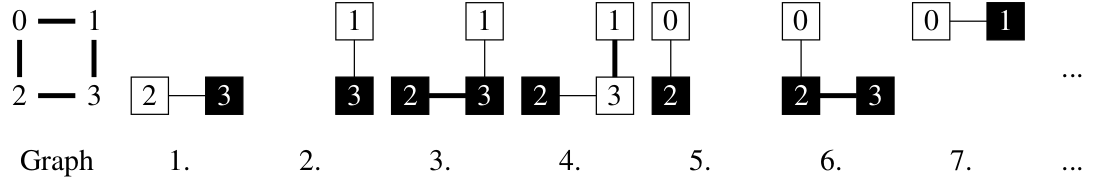
\includegraphics[scale=0.38]{dpccp.png}
	\centering
\end{figure}

\begin{wrapfigure}{R}{0.55\textwidth}
	\vspace{-10pt}
	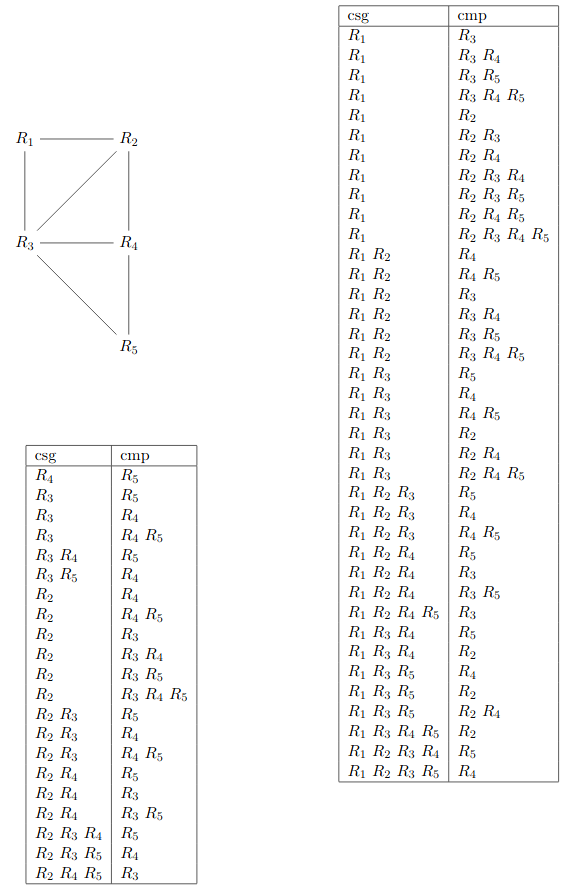
\includegraphics[width=0.55\textwidth]{dpccp_example.png}
	\vspace{-40pt}
\end{wrapfigure}

A total order is achieved by \textbf{labeling nodes} through a breadth-first search. After this preparatory step, the actual algorithm can start having available all nodes along with their \textbf{neighborhood} (nodes reached with an edge). Furthermore, each set has a block composed by nodes coming before, to avoid enumerating twice.

All nodes are considered in descending order and emitted (since each is a connected subgraph), then the graphs are recursively expanded prohibiting nodes with smaller labels. 

Expansion is performed similarly to DP-sub, looking in the neighborhood among possible combinations. The set of valid nodes increases over time, allowing more degrees of freedom.

However, generating connected subsets is not enough: complement pairs have to also be found. First of all, for each $S_1$ all its complements are generated (only once), again using breadth-first, and the procedure is called recursively.

To achieve idealistic runtime, set operations should be performed in constant time, but in the general case this is not expected and a linear delay might happen; in practice, values are encoded as integers to gain speed, yet this only works in the order of 64 relations.

Another solution is using bitsets, implementations with dynamic memory and variable size. This does not guarantee constant time either, even if allocating enough bits should never cause a resize.

\subsection{Complex queries and DPhyp}
There are cases in which the query graph is particularly complicated, such as $abs(r_1.f + r_3.f) = abs(r_4.g + r_6.g)$. This kind of operation generates a hypergraph, connecting more than two relations at once: common algorithms cannot be applied. DPSize does not consider the query graph, so it could be used, but it does not have optimal runtime.

A \textbf{hypergraph} is a non-empty set of nodes and edges where a \textbf{hyperedge} is an unordered pair of non-empty proper subsets with empty intersection. They have a total order via an arbitrary relation, to avoid enumerating multiple times, or breadth-first search.

DPhyp extends DPccp in the following way:
\begin{enumerate}
	\item Constructing connected complement pairs;
	\item Connects subgraphs and complement pairs by recursively traversing the graph;
	\item Connected subgraphs are increased by following edges to neighboring nodes, interpreting hyperedges as $n : 1$ edges leading from $n$ of one side to one.
\end{enumerate}

The approach is similar as for regular graphs, starting with one node and recursively expanding. However, hyperedges have a many-to-many relationship, and an additional choice of where to expand must be taken, while still guaranteeing DP order. The DP table can be tested to check if nodes into subsets are connected, implying an entry already exists. 

For instance, it is impossible to join a set of relations with only one relation which is connected by a hyperedge, since it means some information is lacking and a cross product would be necessary. Therefore, the single relation is recursively expanded checking for connections.

A minor change to solve this issue is choosing a representative for each hyperedge (\textit{canonical end node}, the 1), leading to the last node in total order, so that duplicates are prevented. Checks for connectedness are still required, because this method leads to temporarily disconnected graphs which must be further expanded.

\subsubsection{Non-inner joins}
Another interesting case involves \textbf{non-inner joins} (either outer or unnesting), not freely reorderable (performing an inner join before an outer will reduce the number of output tuples, and vice versa). 

\begin{wrapfigure}{L}{0.4\textwidth}
	\vspace{-15pt}
	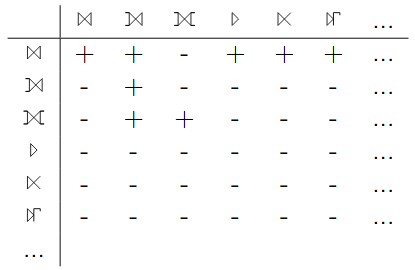
\includegraphics[width=0.4\textwidth]{matrix.png}
	\vspace{-35pt}
\end{wrapfigure}

There are compatibility matrices stating whether two join operations are commutative assuming syntax constraints, i. e. $(R \circ_1 S) \circ_2 T \equiv R \circ_1 (S \circ_2 T)$. For instance, full outer joins can be swapped with themselves. 

Using this information, it is easy to figure out which operations are permitted. Having an expression $E = (R \circ_{p_1} S) \circ_{p_2} T$, it might be transformed into $E' = R \circ_{p_1} (S \circ_{p_2} T)$ and vice versa. If there is a conflict, the ordering is invalid. 

For each operator, the syntactic eligibility set (SES) is built, a set of relations which \textbf{must be in the input} before an expression can be evaluated. It contains the tables referenced by a predicate.

\begin{wrapfigure}{R}{0.5\textwidth}
	\vspace{-5pt}
	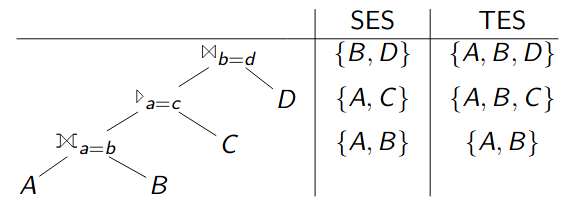
\includegraphics[width=0.5\textwidth]{ses_tes.png}
	\vspace{-35pt}
\end{wrapfigure}

Then, the total eligibility set (TES), capturing syntactic constraints and additional reordability constraints, is constructed in a bottom-up way, starting with SES and checking for conflicts in selectivity. If this is the case, another TES is added, capturing reordering restrictions. 

The output obtained adding TES encodes the necessity of certain relations while constructing hyperedges, eliminating invalid reorderings. TES are used to build hypegraphs and reduce the search space, to directly cover all possible conflicts.

\subsection{Simplifying the query graph}
The dynamic programming approach always considers minimal number of join-pairs, so it is not expected to get a better runtime for exact solutions. The set of possibilities is limited, and algorithms perform slowly for certain query graphs (stars), but the complexity is most likely the best to be achieved.

There are ways to recognize whether the problem is \textbf{too complicated} to be solved with DP, and simplify (from an optimizer point of view) the query graph until it gets tractable. 

The core idea is to \textit{apply safe simplifications before risky ones}. Some possibilities of course are going to be ruled out if edges are removed, hence safe modifications are preferred, using a \textbf{greedy} method for simpler problems and then performing \textbf{DP} on intermediate results. 

However, greedily choosing joins can be really hard in practice, so the chosen approach is to choose joins to \textbf{avoid} first, based on cardinality and selectivity.

To effectively decrease the search space size, some joins (shrinking) can be forced to be performed first, \textit{halving} the number of potential plans with each restriction. 

The steps to be performed are:
\begin{enumerate}
	\item Examine all joins that have a relation in common (\textbf{neighboring}), also considering hyperedges;
	\item Check that a pair can be swapped of order (needs a fast cycle checker, trying to construct a topological ordering);
	\item Compute the \textbf{ordering benefit} with different heuristics;
	\item Retain the pair with \textit{maximal estimated ordering benefit}, maintaining priority queues to speed up repeated simplification;
	\item Return the query graph in which the edge corresponding to the join is changed to a hyperedge.
\end{enumerate}
This method is more restrictive, hence simpler. Repeatedly simplifying graphs allows the complexity of them to decrease monotonically, as each steps adds more restrictions.

The ordering benefit can be estimated in several ways. One approach is to maximize the following:
$$\text{orderingBenefit}(X \bowtie_1 R_1, X \bowtie_2 R_2) = \frac{C((X \bowtie_1 R_1) \bowtie_2 R_2)}{C((X \bowtie_2 R_2) \bowtie_1 R_1)}$$
$C$ is an arbitrary cost function, for instance $C_{out}$ when no other information is available.

The rationale, again, is that if a join is orders of magnitude cheaper than the same join in a different order, it is very likely that the first will come before the second in the optimal solution.

The program should also know when to \textbf{stop} simplifying: this is achieved when memory or time constraints are satisfied, along with counting the number of connected subgraphs or bounding through memory consumption.

Counting is fast, but not immediate, and cannot be performed after every simplification: a reasonable choice is 10 000 connected subgraphs.

The full optimization algorithm runs first of all computing a list of query graphs, in which the elements are the same graph after each step, performing simplifications until a total order is reached; to find a specific plan, binary search is employed and then DPhyp is ran on each of them.

Binary search allows to find the graph with the least number of simplification steps having a complexity $\leq b$, to then store it in the DP table. 

After the optimal simplification is obtained, dynamic programming is used to get the ultimate result.

Simplification heuristics are subject to mistakes, hence performing too many probably means at some point the cost will increase, and it would be best to stop earlier. This problem is NP-hard.

\subsection{Adaptive Query Optimization}
The effectiveness of this method comes from the huge variety of possible queries to be performed in the real world, of which most are small, but some can arrive up to thousands of relations.

Reducing the search space is essential, but greedy algorithms do not perform that well on large graphs. On the other hand, dynamic programming has exponential runtime and a lot of assumptions, so a large search space leads to NP-hard problems. 

Furthermore, \textit{there are no guarantees that running a computationally expensive procedure leads to the best join plan}: often benchmarks fail to represent the real world: a tradeoff between speed and performance is necessary.

To summarize, the decision flow chooses the following approaches, considered to be the state of art of join ordering:
\begin{itemize}
	\item \textbf{Dynamic programming} for easy query graphs:
	\begin{itemize}
		\item DPhyp with $\leq 10k$ DP entries, guaranteeing an optimal plan yet not very powerful:
		\begin{itemize}
			\item Up to 100 relations for chains;
			\item 14 relations for cliques.
		\end{itemize}
		\item GOO/DPhyp if linearization is impossible;
	\end{itemize}
	\item \textbf{LDP} (linearized dynamic programming) for medium ones;
	\item \textbf{Greediness} (still in a limited way, keeping in mind restrictions) to achieve a reasonable optimization time.
\end{itemize}

Complexity is measured with both time and space requirements, and it strictly depends on the structure of the query graph. Once queries become reasonably large, not only the join ordering
algorithm itself plays an important role, but also the implementation
of data structures.

\subsubsection{Search Space Linearization (LDP)}
Search space linearization (LDP) is a technique working for medium-sized and large queries (in the order of a hundred relations, scaling well), always assuming no cross products to improve performance. 

The main goal is to transform a complicated query graph in a \textbf{chain}, since most algorithms perform badly on cliques. Search space is \textit{linearized} by restricting the DP algorithm to consider only \textbf{connected subchains} of a linear relation ordering, instead of arbitrary combinations.

\begin{wrapfigure}{L}{0.6\textwidth}
	\vspace{-18pt}
	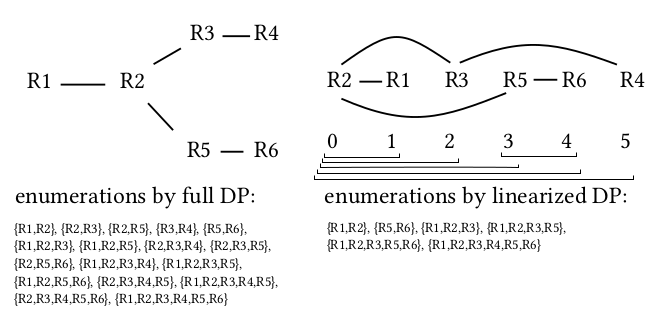
\includegraphics[width=0.6\textwidth]{lindp.png}
	\vspace{-30pt}
\end{wrapfigure}

Unfortunately, hypergraphs cannot be expressed in such a linearized form, hence this algorithm can only be applied to queries that can be represented by a regular graph.

Knowing the order of relations in the optimal plan, LDP generates the optimal plan from the linearization in polynomial time, combining solutions for subchains of increasing size. 

Furthermore, as seen above, the DP table is much smaller.

The way the graph is linearized also has a great impact on the quality of the final plan, thus even if time is greatly reduced, some join orders which may be good are removed.

This is countered knowing the optimal order can be obtained through \textbf{IKKBZ} in quadratic runtime (with eventually applying MST if the graph is cyclic), so it is indeed possible to order relations efficiently. The result is as least as good as the best left-deep plan, and the optimal bushy plan can be discovered with further steps.

However, a runtime of $O(n^3)$ is still too large for wide query graphs, so a \textbf{combined approach} is taken in case of joining more than 100 relations:
\begin{enumerate}
	\item The query plan is build through a greedy algorithm, such as GOO;
	\item The $k$ most expensive trees are iteratively optimized again using dynamic programming.
\end{enumerate}

The latter algorithm is indeed LDP: most DP approaches would need a relatively small $k$ to achieve reasonable time, while LDP allows to increase the factor $k$ up to 100.

This way, there is more freedom to correct mistakes the greedy phase has introduced, as relations can move up to 100 places within the tree. For small number of relations, however, DPhyp still performs the best. 

\subsection{Generating Permutations}
Generating permutation is a \textit{lightweight} algorithm: it does not require a DP table, and the solution can be found even without completing the enumeration of possibilities. This allows very low space consumption, imposing \textbf{stricter time requirements} (stop if time runs out).

Generating all permutations is too expensive, but some of them can be ignored: if a join is more efficient than another, the latter can be discarded.

This can be achieved considering left-deep trees: those are permutations of the relations to be joined, which can be generated directly. To make the process cheaper, some permutations can be ignored once again applying the DP reasoning (if a solution is better than another, there is no point extending the latter).

\textit{A sequence is only explored if exchanging the last two relations does not result in a cheaper alternative. }

The algorithm performs a recursive search while comparing the costs of adding a relation in the end or earlier in the chain, making the optimal plan better after each iteration. 

This process is implemented considering a \textbf{prefix} $P$ and the rest $R$, increasing $P$ recursively and keeping track of the best tree found so far. 

Since modifications are performed in-place, the occupied memory is linear; however, it potentially runs for a long time, and some constraints need to be placed. An instance of the worst case scenario is when a \textbf{tie} occurs, since the algorithm must explore both alternatives. 

\subsection{Transformative Approaches}
This technique is used among modern commercial DBMS (Microsoft SQL server), but it is likely not the best approach. The main idea is to directly apply properties and equivalences to construct new query plans, yet this raises plenty of problems: there is no order, the optimal solution must be guaranteed and such.

The algorithm is presented as a transformation-based enumeration to avoid the generation of duplicates, to obtain a lower bound for the number of combinations, employing both \textbf{memoization} and \textbf{transformation rules}.

This works as follows:
\begin{enumerate}
	\item A set of visited plans is kept, starting with a simple expression;
	\item All transformation rules are applied to visited plans, adding the result to the set if they are new;
	\item When no new plans can be generated, the complete search space has been explored.
\end{enumerate}

Commonly used sets of transformations are:
\begin{itemize}
	\item RS-B0 (one of the properties is redundant):
	\begin{itemize}
		\item Right associativity: $(A \bowtie B) \bowtie C \rightarrow A \bowtie (B \bowtie C)$;
		\item Left associativity: $A \bowtie (B \bowtie C) \rightarrow (A \bowtie B) \bowtie C$;
		\item Commutativity: $A \bowtie B \rightarrow B \bowtie A$;
	\end{itemize}
	\item RS-B1 (not redundant anymore):
	\begin{itemize}
		\item Left associativity: $A \bowtie (B \bowtie C) \rightarrow (A \bowtie B) \bowtie C$;
		\item Commutativity: $A \bowtie B \rightarrow B \bowtie A$;
	\end{itemize}
	\item RS-L1, for left-deep trees:
	\begin{itemize}
		\item Swap: $(A \bowtie B) \bowtie C \rightarrow (A \bowtie C) \bowtie B$;
		\item Bottom commutativity: $B_1 \bowtie B_2 \rightarrow B_2 \bowtie B_1$, for base tables (underlying tables storing metadata for a database);
	\end{itemize}
	\item RS-B2, to avoid duplicates:
	\begin{itemize}
		\item Commutativity: $A \bowtie_0 B \rightarrow B \bowtie_1 A$, disabling all other rules for the new operator $\bowtie_1$;
		\item Right associativity: $(A \bowtie_0 B) \bowtie_1 C \rightarrow A \bowtie_2 (B \bowtie_3 C)$, disabling associativity and exchange on $\bowtie_2$;
		\item Left associativity: $A \bowtie_0 (B \bowtie_1 C) \rightarrow (A \bowtie_2 B) \bowtie_3 C$, disabling associativity and exchange on $\bowtie_3$;
		\item Exchange: $(A \bowtie_0 B) \bowtie_1 (C \bowtie_2 D) \rightarrow (A \bowtie_3 C) \bowtie_4 (B \bowtie_5 D)$, disabling all other rules for application on $\bowtie_4$.
	\end{itemize}
\end{itemize}

Furthermore, two arbitrary relations can be swapped, or cyclic rotations can be performed. It is possible to obtain the optimal solution just applying RS-0, however the other rules allow a smaller number of steps hence a quicker runtime.

In practice, the output is easily suboptimal: the whole search space is to be considered and the same plan can be generated more than once. 

A memoization approach is therefore introduced to remember the intermediate solutions, using pointers to class and expanding their relative members. Replication is avoided by using \textit{shared copies} only, organizing a network of \textit{equivalence classes}.

Each class is a set of operators which all produce the same result, and each operator takes a class as input, meaning that any operator in that class may be applied. A hash table is furthermore used to speed up finding results.

\textbf{RS-B2} is the only set of rules which effectively avoids duplicates, working with the following logic: some rules should not be applied twice, since their output will be redundant (e. g. commutativity).

The applicability of a rule can be encoded using a single bit, which is not a huge overhead in memory. Even with restrictions, RS-B2 rules generate all valid bushy join orders.

Linear trees can also be obtained employing a variant of this, using only associativity and commutativity.

\subsection{Generating Random Join Trees}
Constructing a \textbf{random join tree} is quite useful in practice: assuming the cost is random, it is possible to find a solution which is really close to the optimal one, and allows to get information about the distribution.

In this case, considering cross products make the problem simpler, but the \textit{uniformity of join trees} (having the same probability for each tree) is a challenge.

To help this, the concepts of \textbf{ranking} and \textbf{unranking} are introduced:
\begin{itemize}
	\item A ranking is a mapping $f : S \rightarrow [0, n[$;
	\item An unranking is a mapping $f : [0, n[ \rightarrow S$.
\end{itemize}
The idea is to generate random numbers, to then map them to the and the function must also be able to unrank in a fast way.

A trivial mapping would just be generating all possible trees and incrementing a counter, but this method is not efficient: the solution set should be smaller.

Random permutations can be applied as a starting point for the algorithm, shuffling an array (for each element in descending order, swap it with a random one up to its position) to generate a left-deep tree. 

In the first call, there are $n$ choices of random elements $r_{n-1}, \dots, r_0$ where $0 \leq r_i \leq i$, in the second one there are $n - 1$ and so on, obtaining a number of $n!$ sequences with an one-to-one relationship with the set of all permutations.

Unranking works trying to find a sequence from the initial value, which is independent from previous ones: $r_{n-1} \equiv r \mod n$ is set, and the swap is performed. $r' = \lfloor r/n\rfloor$ is defined and iteratively unranked to construct a permutation of $n - 1$ elements. 

\textbf{Bushy trees} are obtained in a similar way, yet using a Catalan number $b$ (the amount of different trees) to obtain the relations, and applying the previous procedure with another random value $p$ smaller than $n!$. Unranking works attaching the relations in order $p$.

To encode trees, whenever an inner node is encountered a left bracket (1) is added, and when a leaf node is encountered a right bracket (0) is added, except for the last one. Brackets are then substituted with the respective binary value, and the relations correspond to the position of 1s starting from left. 

Unranking binary trees also has an unique correspondence with Dyck words (sequences with proper brackets): to count how many possibilities are there, it is possible to plot them knowing that the first character must be a left bracket, and last one a right bracket. A tree is any path in the grid from $(0, 0)$ to $(2n, 0)$.

\begin{wrapfigure}{L}{0.6\textwidth}
	\vspace{-10pt}
	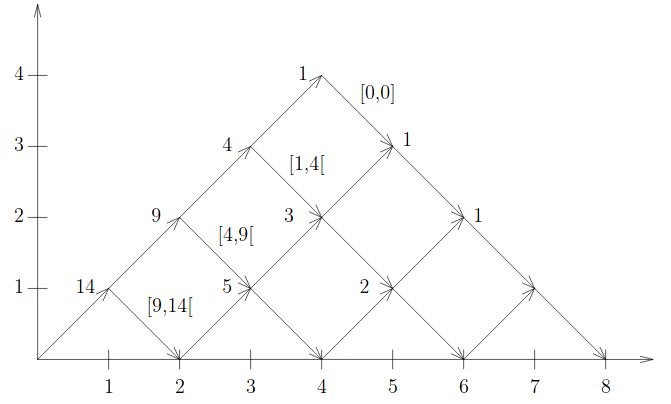
\includegraphics[width=0.6\textwidth]{grid.png}
	\vspace{-30pt}
\end{wrapfigure}

The number of different paths from $(0, 0)$ to $(i, j)$ can be computed with the following formula:
$$p(i, j) = \frac{j+1}{i+1} {{i+1}\choose{\frac{1}{2}(i+j)+1}}$$
These numbers are the \textit{Ballot numbers} (useful for elections!). Hence, all the paths from beginning to end are $p(2n - i, j)$, which is indeed a Catalan number. Choices which have not been taken are subtracted by the rank at each iteration.

If the number of paths does not exceed the rank, a parenthesis is open and the grid is traversed upwards. When it does, a parenthesis is closed and a step down is taken, \textbf{decrementing} the rank by the number of excluded paths.

The decision of upwards or downwards is as easy as flipping a coin, but this does not respect a uniform probability since there are more trees starting with a left brackets, and going down is not possible in all cases. 

The procedure works in five steps:
\begin{enumerate}
	\item List merges (notation, specification);
	\item Join tree construction;
	\item Standard Decomposition Graph;
	\item Counting;
	\item Unranking.
\end{enumerate}
A list $l'$ is the projection of a list $L$ on $P$ if $l'$ contains all the elements of $L$ respecting $P$ in the same order. A list merge $L$ is the union of two disjoint lists, both obtained from $L$.

A merge of two lists whose respective lengths are $l_1$ and $l_2$ is equivalent to an array of non-negative integers whose sum is equal to $l_1$. 

Therefore, the number of decomposition of any non-negative integer in a sequence of non-negative integers with $\sum_{i=1}^{k} \alpha_k = n$ is ${n+k-1}\choose{k-1}$.

The number of possible merges is ${l_1+l_2}\choose{l_2}$, but this is too expensive to be computed all the iterations, hence it is split in two parts which are then materialized. 

To establish a bijection, the set $S$ is partitioned into disjoint smaller sets: when ranking $x \in S_k$, first the local rank is computed, obtaining $rank(x) = \sum_{i=0}^{k-1} \abs{S_i} + local-rank(x, S_k)$.

The rank can be interpreted as the number of elements in every previous bucket which have not been chosen plus the local ordering of the element in the current set. 

Unranking simply consists in computing $r' = r - \sum_{i=0}^{k-1} \abs{S_i}$, i. e. subtracting all the partitions which have not been taken yet. 

Each possible merge is partitioned into subsets, each having an increasing number of elements. In each of them, there are $M(l_1 - j, l_2 - 1)$ elements. To unrank a value, its partition is firstly computed, setting $k = min_j r \leq \sum_{i=0}^{j} M(j, l_2 - 1)$ and $\alpha_0 = l_1 - k$. The new rank is then updated and used for the next iteration.

If the query graph is cyclic, there does not exist a way to generate trees with random probability; not allowing cross products implies choosing only relationships which are \textbf{connected}, introducing bias. 

Another representation of join trees works through \textbf{anchored lists}:
\begin{itemize}
	\item If $T$ is a single leaf node, then $L = <>$;
	\item if $T = T_1 \bowtie T_2$ and a leaf $v$ occurs in $T_2$, then $L = <T_1 | L_2>$ where $L_2$ is the anchored list representation of $T_2$.
\end{itemize}
Here, left and right are not distinguished, since there is no way to remember the direction. Leafs are inserted introducing insertion pairs, couples $(T', k)$ of lists and rank in which only one node (missing from $T$) is inserted at position $k$. This is a bijective mapping.

\newpage
\subsubsection{Standard Decomposition Graph}
\begin{wrapfigure}{R}{0.55\textwidth}
	\vspace{-5pt}
	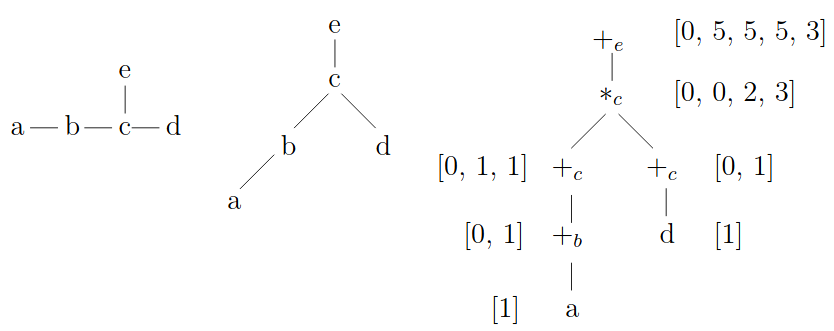
\includegraphics[width=0.55\textwidth]{std.png}
	\vspace{-70pt}
\end{wrapfigure}
A STD describes the possible constructions of join trees. It uses two kind of nodes:
\begin{itemize}
	\item $+$ for \textbf{leaf} insertion;
	\item $*_w$ for merging \textbf{subtrees} whose only common leaf is $w$.
\end{itemize}
This is done with three steps:
\begin{enumerate}
	\item Picking an arbitrary root node;
	\item Transforming the query graph into a tree;
	\item Calling the algorithm which turns the query graph into a SDG, looking at how many child nodes there are and performing leaf insertions with one input, else merging to obtain two new $+$ nodes.
\end{enumerate}

\subsection{QuickPick}
QuickPick is useful to have a first insight into what the search space looks like, building pseudo-random trees by randomly select edges. This algorithm is easy to implement and quite fast, however it loses uniformity: the usual way to take advantage of it is running it multiple times and picking the best output.

It works without cross products, since each edge must join two relations, and can output any kind of tree shape. The key element of the algorithm is sampling from a \textbf{mapping} of randomly generated sequences of join predicates to query plans.

Query plans are constructed in a bottom-up way, simultaneously computing the costs and discarding partial plans as soon as they exceed the best costs found so far. 

QuickPick performs biased sampling by selecting edges from the join graph and adding the respective joins to the query plan. 

After this step, if either the plan is complete or the cost exceeds the best plan so far, the query plan is \textbf{reset}, eventually updating the cost if a better alternative has been found.

The procedure only ends when the stopping criterion is fulfilled, usually an amount of time or operations. However, QuickPick tends to \textbf{converge} due to its biased cost distribution.

There is a variant starting with all possible sets of trees and randomly joining them by selecting an edge. If an edge connects two subtrees, it is replaced with a join, removing the two subtrees until only one tree is left. 

Failure can happen if cycles exist in the graph. Furthermore, some trees are more likely to exist than others, since sometimes swapping two edges makes no difference among the structure.

To check whether an edge connects two relations in different subtrees, an approach similar to Kruskal's algorithm is used: through an union-find data structure it is possible to do this efficiently.

\subsection{Metaheuristics}
Metaheuristics are general optimization strategies working well for even large problems, but are unaware of the real issue and just rely on computational power.

Formally, \textit{a \textbf{metaheuristic} is a higher-level procedure or heuristic designed to find, generate, or select a heuristic (partial search algorithm) that may provide a sufficiently good solution to an optimization problem, especially with incomplete or imperfect information or limited computation capacity.}

By searching over a large set of feasible solutions, they can often find good solutions with less computational effort than optimization algorithms, iterative methods, or simple heuristics.

It is not proven how well they perform or what kind of problem they solve, but they are widely used by modern DBMS.

\subsubsection{Iterative Dynamic Programming}
The main idea of IDP is to apply dynamic programming several times
in the process of optimizing a query, either to optimize different parts of a plan
separately or in different phases of the optimization process.

This approach generally works better than simple dynamic programming variants, since when the query it simple the plan will be the same, and it scales better than naive algorithms. It also considers memory limitations, eventually restarting if it exceeds a threshold and using previous results as building blocks. 

The iterative improvement approach starts with a \textbf{random tree}, applies some rules to improve (e. g. transformative approaches) and stops only when no further improvement is possible. If the tree after random modifications gets worse, the change is undone. 

Improvements, therefore, are applied both on a query graph and a tree basis, trying several trees and randomly optimizing each of them.

Metaheuristics work trying to find an optimal, and have the consequence of risking to get stuck into a local minimum: usually a time limit is implemented so that the procedure always terminates, and there are different start points to generate multiple results.

Cross products could be generated by accidentally swapping two relations which are not linked, hence a method similar to QuickPick is used, manipulating edges instead of nodes.

IKKBZ can be used with an acyclic query graph to obtain the optimal left-deep tree, which is then compared with the iterative improvement result.

\subsubsection{Simulated annealing}
Simulated annealing is another approach which allows moving from a local minimum even if the solution gets worse, defining a \textbf{probability} based on the temperature for the worse tree to be swapped with the current best one. 

The only problem is \textit{optimizing temperature and time}, picking initial values and thresholds to decrease or rise the temperature, yet there are some rule of thumbs working well in practice.

Simulating annealing is often used along with iterative improvement, using the latter to find a local minima and the former to try and find a better plan.

\subsubsection{Tabu search}
Tabu search sets some nodes in the graph as \textbf{forbidden}, to extend the search space trying to find different solutions. The cheapest results among all neighbors are chosen, even if they are worse than the current one, forcing the algorithm to never go back. This is useful to avoid cycles.  

Size of the tabu set is fixed, otherwise it might eventually contain all the relations: whenever the size is exceeded, the oldest node is removed and allowed back into the search space. 

\subsubsection{Genetic algorithms}
Genetic algorithm, employed in PostgreSQL [\href{https://www.postgresql.org/docs/current/geqo.html}{source}], is a heuristic optimization method operating through randomized search. It functions in the same way as a population model, based on \textit{survival of the fittest}. Join trees are elements which generate successors by \textbf{crossover} or \textbf{mutation}, only keeping the best trees.

The coordinates of an individual in the search space are represented by chromosomes, in essence a set of character strings. A gene is a subsection of a chromosome which encodes the value of a single parameter being optimized.

Through simulation of the evolutionary operations, new generations of search points are found that show a higher average fitness than their ancestors. 

Query optimization in this case is approached as it was the TSP problem, implementing steady state (replacement only of the least fit individuals) and edge recombination crossover for fast convergence. 

The algorithm works with the following process:
\begin{enumerate}
	\item The standard planner generates plans for scans of individual relations;
	\item Transforms each join plan into a sequence, and estimates its cost;
	\item Least fit candidates (more expensive) are discarded;
	\item New candidates are generated by combining genes, i. e. using random portions of low-cost joins to create new sequences.
\end{enumerate}

The problem with this simulation is finding an encoding between trees and population, especially representing crossover and mutation. There are two different possibilities: 
\begin{itemize}
	\item \textbf{Ordered list}, showing a tree as a permutation of numbers and joining them from left to right, implementing the bushy variant naming edges instead of nodes;
	\item \textbf{Ordinal number}, starting with a natural order:
	\begin{itemize}
		\item For left-deep trees, finding the index of the first relation to be joined, setting the first character in the chromosome string as $i$ and removing it from the list;
		\item For bushy trees, encoding in bottom-up, left-to-right, looking at two positions at once and again removing them, but replacing them with a third symbol to describe the tree.
	\end{itemize}
\end{itemize}
Crossover is simulated either by \textbf{subsequence} exchange or \textbf{subset} exchange, generating permutations such that the order of appearance is respected or simply swapping elements of equal length.

\begin{wrapfigure}{R}{0.6\textwidth}
	\vspace{-18pt}
	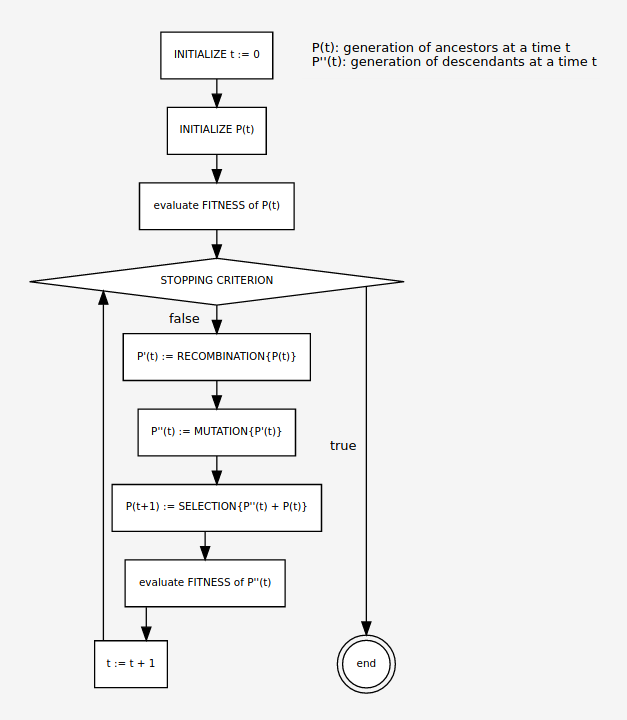
\includegraphics[width=0.6\textwidth]{genetic.png}
	\vspace{-60pt}
\end{wrapfigure}

An example of crossover by subsequence exchange is:
\begin{enumerate}
	\item Assuming two individuals with chromosomes $u_1v_1w_1$ and $u_2v_2w_2$;
	\item Taking $v$ and permuting its relations to obtain $u_1v'_1w_1$, $u_2v'_2w_2$.
\end{enumerate}

A mutation, on the other hand, \textit{randomly alters} a character in the encoding, hence a swap can be considered a mutation as well.

The algorithm is implemented with a \textbf{selection} phase: population is sorted according to survival probability (sorting trees by cost and keeping the best) and some of them are selected to be subject of crossover or mutations.

Since crossover increases the population, selection needs to be performed again until the maximum number of iterations or the given size are reached.

Like other metaheuristics, parameters rely on human hand-made benchmarking.

\section{Accessing the data}
Optimization has also a \textbf{hardware} component: accessing the data has to be done efficiently, measuring and modeling physical costs. 

\begin{wrapfigure}{L}{0.55\textwidth}
	\vspace{-15pt}
	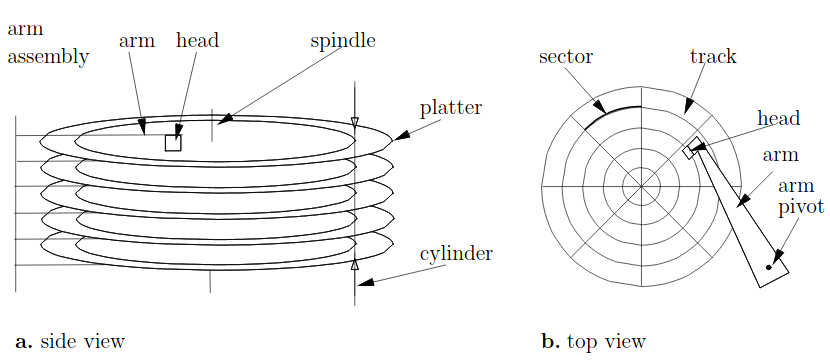
\includegraphics[width=0.55\textwidth]{disk.png}
	\vspace{-25pt}
\end{wrapfigure}

Older devices store memory in a stack of \textit{rotating disks} on which an arm writes data with its head. Each disk is divided in \textbf{tracks} and \textbf{sectors}, of which the outer are longer than the inner.

Cylinders are organized in zones: each of them contains a fixed number of consecutive cylinders, with the same amount of sectors per track. 

Since the disk is rotating, the throughput is higher on outer cylinders, and reading is only possible where the head is, making this operation quite slow since it is impossible to jump. On SSD, this is indeed implemented.

A good approximation of the \textbf{seek time} among $d$ cylinders is:
$$seektime(d) = \begin{cases}
	c_1 + c_2\sqrt{d} & d \leq c_0 \\
	c_3 + c_4d & d> c_0
\end{cases}$$
Constants indicate the maximum number of cylinders where no coast take place, i. e. the point in which the head can be efficient. 

The square is introduced because in the low part of hardware the distance is less, hence the head moves faster. On the other hand, the formula is linear if the distance is short.

Since the current position on the disk is unpredictable, it is difficult to produce single cot estimation, however modeling many accesses gives a somewhat accurate measurement. 

\begin{wrapfigure}{R}{0.5\textwidth}
	\vspace{-15pt}
	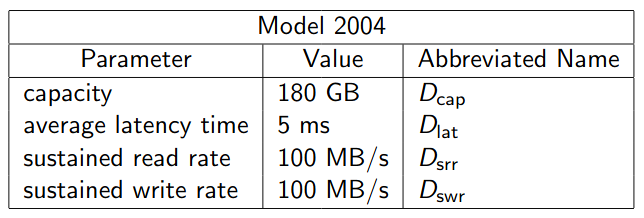
\includegraphics[width=0.5\textwidth]{parameters.png}
	\vspace{-30pt}
\end{wrapfigure}

Parameters are aggregated, introducing average latency time (for positioning) and sustained read/write assuming a sequential scan. 

The time a disk needs to read and transfer $n$ bytes is approximately $D_{lat} + \frac{n}{D_{srr}}$. Examples of these values are given in the table.

Database developers, as introduced before, distinguish between \textbf{random} and \textbf{sequential} access. The latter is faster, since it assumes data only needs to be \textit{read in sequence} after finding its position, while a random access implies seeking the location of each page (the smallest portion which can be read, generally 8kb).

Example: to read 100MB, sequential read takes $5ms + 1ms$, while random read has to scan 8k pages and takes $65s$.

This has consequences in practice: for instance, an index may be efficient only if a \textit{small portion of the data is accessed}, else there is a risk for the whole structure to be traversed with a random access behavior. On the other hand, it could be expensive to perform a scan if there are many pages involved. 

\subsection{Counting the number of accesses}
A proposed cost function to calculate sequential scan time is: 
$$5ms + \frac{\abs{page\_size}}{\abs{bandwidth}} * \#pages$$
Now, the problem becomes estimating the bandwidth, the number of needed pages and their cost. These can vary between different use cases, or be influenced by indexes. 

More parameters are introduced for a better overview, assuming a uniform distribution of the tuples:
\begin{itemize}
	\item $N$, number of tuples (items) in relation $R$;
	\item $m$, number of pages (buckets) in which tuples of $R$ are stored ($m = 1$ all pages are accessed);
	\item $B = \frac{N}{m}$, tuples for page (blocking factor);
	\item $k$, number of distinct TID ($k = 1$ implies one page is accessed).
\end{itemize}
The probability to request a set with $k$ items is $\frac{1}{{{N}\choose{k}}}$, because of the uniformity assumption.

\subsubsection{Yao's formula (direct, uniform, distinct)}
Considering $m$ buckets with $n$ items, then there is a total of $N = nm$ items. Randomly selecting $k$ \textbf{distinct} items give a number of qualifying buckets which is:

$$\bar{y}^{N, m}_n(k) = m * y^N_n(k)$$
$$y^N_n(k) = \begin{cases}
	[1 - p] & k \leq N - n \\
	1 & k > N - n
\end{cases}$$
$y^N_n(k)$ is the probability that bucket $n$ contains at least one tuple, and $p$ is the probability that a bucket contains none of the $k$ items.
\begin{wrapfigure}{R}{0.25\textwidth}
	\vspace{-25pt}
	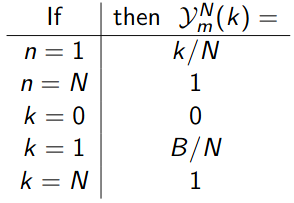
\includegraphics[width=0.25\textwidth]{yao.png}
	\vspace{-30pt}
\end{wrapfigure}
$$p \quad = \quad \frac{{{N-n}\choose{k}}}{{{N}\choose{k}}} \quad = \quad \prod_{i=0}^{k-1} \frac{N-n-i}{N-i} \quad = \quad \prod_{i=0}^{n-1}\frac{N-k-i}{N-i}$$
These formulas are useful to avoid computing $N!$, which is too expensive to do in practice. The choice of formula depends on $N$ and $k$.

However, even with simplifications, calculations are not cheap, and fractions may not be integers: further steps must be taken, such as introduction of a Gamma function and approximations (\textbf{Waters}):
$$p \approx \Big( 1 - \frac{k}{N} \Big)^n$$
This works implying there is a fraction of $\frac{k}{N}$ tuples which are relevant for the query, multiplied for the number of pages. The problem here is, if the first tuple does not qualify, the likelihood that a latter one qualifies increases (there is less space); in general, probability is not uniform.

The estimation is roughly accurate with $N >> n$, and much cheaper to compute. There are other formulas which are simpler, but more complicated to express (\textbf{Bernstein}):
$$y_n^{N,m}(k) \approx \begin{cases}
	k & k < \frac{m}{2} \\
	\frac{k+m}{3} & \frac{m}{2} \leq k \leq 2m \\
	m & 2m \leq k
\end{cases}$$
This evaluation tries to interpolate $k$ depending on its comparison with $m$, and is faster to compute. Each case is plausible, yet not very precise. 

Dihr and Saharia computed some upper and lower bounds for $p$, claiming these are accurate with a minimal difference from real-case scenarios.

\subsubsection{Cheung's formula (direct, uniform, non-distinct)}
Index nested loop joins often involve reading the same tuple multiple times, fetching join partners using the index. This strategy uses very little memory, with time linear in the left side.

In this case, Yao's formula is not sufficient, and a \textbf{multiset} (set with duplicates) approach is introduced. The number of multiset with cardinality $k$ containing only elements from a set $S$ with $\abs{S} = N$ is:
$${N+k-1}\choose{k}$$

This works transforming a multiset into a set by summing a crescent value from 1 to $(k-1)$ to each element, making them unique. The other way around applies subtraction. 

Cheung's formula is an extension of Yao's formula considering multisets (not necessarily distinct items among $k$):
$$\overline{Cheung}^{N, m}_n(k) = m * Cheung^N_n \qquad Cheung^N_n(k) = [1 - \tilde{p}] \qquad \tilde{p} \approx \Big( 1 - \frac{n}{N}\Big)^k$$
$$\tilde{p} \quad = \quad \frac{{n-n+k-1\choose k}}{{n+k-1\choose k}} \quad = \quad \prod_{i=0}^{k-1} \frac{N-n+i}{N+i} \quad = \quad \prod_{i=0}^{n-1} \frac{N-1-i}{N-1+k-i}$$
This just expands binomials using the duplicates property. The approximation of $p$ (\textbf{Cardenas}) is derived assuming there are $1 - \frac{n}{N}$ tuples on the current page and applying the power.

The number of \textbf{distinct} values in a $k$-multiset of cardinality $N$ with uniform distribution is:
$$D(n, k) = \frac{Nk}{N + k - 1}$$
This follows by previous statements, expanding the binomial coefficient. This allows to do a simplification (\textit{model switching}), i. e. using Yao's formula after removing duplicates. 

Non-uniform distributions work similarly, yet modeling each probability to access a group of buckets, using summation instead of product. 

\subsection{Sequential accesses on disk}
Accesses on disk are relevant to estimate the cost of \textbf{jumping between two pages or cylinders}: this directly depends on the distance gap. When estimating seek costs, there must be a probability distribution for the distances.  

Assuming the situation is a \textbf{bitvector} of length $B$ with $b$ bits set to 1, then $B - b$ bits are zero, and the accesses can be modeled with $B$ corresponding to the number of cylinders while $b$ indicates that a cylinder qualifies.

Then, the probability distribution of the number $j$ of zeros between two consecutive ones, before the first or after the last is:
$$B^B_b(j) = \frac{{B-j-1\choose b-1}}{{B\choose b}} = \frac{b}{B-j}\prod_{i=0}^{j-1} \Big( 1 - \frac{b}{B - i}\Big)$$
The distance between two ones is obtained taking the expected value of the number of zeros, and adding one for the potential first or last position.

Some other values can be deduced from this, such as the total number of bits from the first bit to the last one (extremes included), which is:
$$B_{tot}(B, b) = \frac{Bb + b}{b + 1}$$
All these computations have several real-life applications: the original motivation implies retrieving values from a B-tree and accessing them on disk, sorting the entries to avoid multiple random lookups. A bitvector module gives information about the distance between pages, to understand how expensive a fetch can be.

\section{Selectivity estimations}
Selectivity estimation has always been assumed to be known until now, yet it is a statistic which needs to be computed, since it is essential for query optimization.

Unfortunately, this is a \textit{fundamentally difficult problem}, and can take quite a long time.

Specifically, there are different selectivity problems requiring different approaches. For arbitrarily difficult queries it is impossible to make an estimation, yet the following three are the most common:

\begin{lstlisting}[language=SQL]
SELECT *
FROM relation r
WHERE r.a = 10
	
SELECT *
FROM relation r
WHERE r.b > 2
	
SELECT *
FROM relation1 r1, relation2 r2
WHERE r1.a = r2.b
\end{lstlisting}

\subsection{Heuristic estimations}
There are some textbook estimations which are not advanced strategies, depending on the predicate.

\begin{wrapfigure}{R}{0.6\textwidth}
	\vspace{-20pt}
	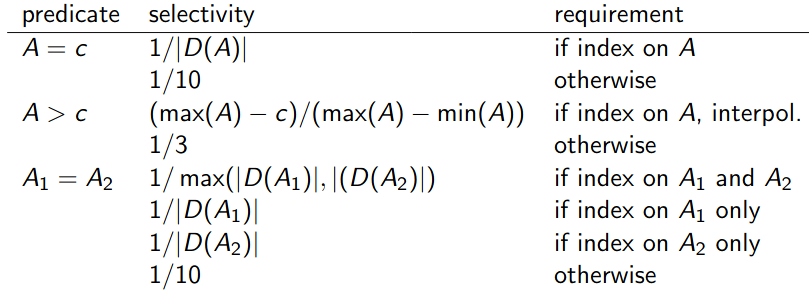
\includegraphics[width=0.6\textwidth]{selectivity.png}
	\vspace{-30pt}
\end{wrapfigure}

Knowing the domain of $A$, for instance, can happen when the column has an \textbf{index}, yet an uniform distribution must be assumed.

Having a range query is also helped by an index, since this additional data structure stores the minimum and maximum value, hence selection can be obtained by interpolation. 

Joins again depend on indices and domain of the involved tables.

\subsection{Building histograms}
Heuristics are quite simple and have the restriction of uniform distribution, so multiple DBMS employ histograms: aggregated data is \textbf{partitioned in buckets} such that $H_A(b) = |\{r\ |\ r \in R \;and R.A \in b\}|$ and thus $\sum_{b \in B} H_A(b) = \abs{R}$.

This methods leads to a much better estimation than previous ones, and computing histograms is also easy since it only involves a sequential scan: the real challenge is selecting the appropriate $B$.

Assuming data is already in buckets, there are formulas giving the appropriate result, applying linear interpolation to the newly obtained histogram:
$$A = c \quad \frac{\sum_{b \in B:c \in b H_A(b)}}{\sum_{b \in B}H_A(b)}$$
$$A > c \quad \frac{\sum_{b \in B:c \in b \frac{max(b) - c}{max(b) - min(b)} H_A(b) + \sum_{b \in B:min(b) > c} H_A(b)}}{\sum_{b \in B}H_A(b)}$$
$$A_1 = A_2 \quad \frac{\sum_{b_1 \in B_1, b_2 \in B_2, b' = b_1 \cap b_2: b' \neq \emptyset} \frac{max(b') - min(b')}{max(b_1) - min(b_1)} H_{A_1}(b_1) \frac{max(b') - min(b')}{max(b_2) - min(b_2)} H_{A_2}(b_2)}{\sum_{b_1 \in B_1}H_{A_1}(b_1) \sum_{b_2 \in B_2}H_{A_2}(b_2)}$$

These computations only give an upper bound, while the lower bound can be up to zero, and it is impossible to predict. Furthermore, the upper bound can be quite an overestimation in the first case, which represents only a rough approximation.

The problem comes from the restriction in the mathematical meaning of $P(A = c) = 0$, which gives a sound result when $A > c$ but fails when the query involves equality. Joining works using some assumptions as well, such as independence.

\subsubsection{Equiwidth}
Building histograms concerns the previously mentioned issue: finding the optimal number of buckets. Typically, this is a fixed value, and it has to work with an unknown distribution.

One particular strategy is partitioning the domain into buckets of equal width, simply constructing them from left to right. This is easy to compute, since it does not require boundaries: it is enough to store minimum, maximum and size. 

However, it fails when data is skewed, causing uneven buckets and therefore a greater estimation error. 

\subsubsection{Equidepth}
Another method is the equidepth, forcing each bucket to have the same number of elements, adopting to data distribution. This technique is very common and not too time consuming, so it is widely used in practice.

The only disadvantages are having to sort the values beforehand, and store boundaries and ties (obviously not the count).

\subsubsection{Interpolation}
Interpolation is a technique to improve accuracy, however it can be difficult to interpolate a histogram: a potential solution is using the distribution function instead, which is continuous and monotonic. This works particularly well in the case $A > c$.

Further research includes analyzing correlations, multi-dimensional histograms and cardinality estimators.

\end{document}